\chapter{Lemmatisation}
\label{sec:lemmatiseurs}

\section{Introduction}
\label{subsec:lemma_intro}

Afin de traiter un texte et d'établir des statistiques sur celui-ci, il est courant de le lemmatiser. La lemmatisation d'un texte, et \textit{a fortiori} d'un mot, correspond à sa transformation en une forme canonique, le \textit{lemme}. Traditionnellement identique à la forme d'entrée d'un dictionnaire, le lemme permet de rassembler sous une même étiquette l'ensemble des flexions et variations graphiques qu'il peut connaître. Pour le latin, il s'agira de rassembler ensemble \textsc{me} et \textsc{mihi} sous une racine commune \textsc{ego}. Cet étiquetage permet de clarifier le signal statistique en éliminant où cela est nécessaire un bruit inhérent aux langues flexionnelles (voire aux langues dont l'orthographe est variable ou localement influencé, commen l'ancien francais ou le latin des inscriptions). Son utilisation principale a longtemps eu pour but la capacité à trouver dans un texte les occurences d'un terme puis a permis la développement plus tardivement de la linguistique de corpus\footcite{mellet2002atouts}.

\subsection{Tâches et définitions générales}

La lemmatisation est donc un effort de traduction d'un texte en un ensemble de formes normalisées, de telle facon qu'\textit{un mot} ne doit connaître qu'une seule annotation de lemme. Cette définition exclut \textit{ipso facto} les outils d'analyse du vocabulaire tels que Collatinus. En effet, ce dernier ne propose pas un étiquettage unique mais un ensemble de possibilités pour chacun des éléments trouvés dans le texte. Pour exemple, là où \textsc{est} est identifiable comme \textsc{edo} et \textsc{sum} par collatinus, un lemmatiseur fait un choix unique, lié généralement au contexte et à la probabilité d'un des deux lemmes d'apparaître à cet endroit.

Enfin, dans le cadre de la lemmatisation, on préfèra l'utilisation du terme "token" à celui de "mot". Un token est un élément qui correspond au niveau le plus bas à la fois aux mots, aux nombres, aux enclitiques pour le latin mais aussi aux signes de ponctuations, et au niveau le plus haut aux phrases. La \textit{tokenisation} consiste donc au découpage d'un texte en un ensemble d'éléments qui seront ensuite la source d'une analyse ou d'un pré-traitement. Pour le latin, la tokenisation cherchera donc à extraire les enclitiques: \mintinline{python}{"lascivusque"} se découpera ainsi en \mintinline{python}{["lascivus", "-que"]}. Ce travail est d'autant plus important qu'il peut faire une différence notable dans le cadre de l'annotation: ainsi, identifier \mintinline{python}{"P. Naso."} en \mintinline{python}{["P", ".", "Naso", "."]} induira une rupture de syntaxe sur le premier "." à travers la création d'une nouvelle phrase là où \mintinline{python}{["P.", "Naso", "."]} indiquera une abréviation.

Au delà de la lemmatisation, deux autres tâches sont souvent adjointes: elles correspondent à des informations syntaxiques et morphosyntaxiques liées aux tokens. D'une part, on adjoint en général à la lemmatisation une Part-Of-Speech (POS). Cette tâche est traitée très rapidement par les annotateurs automatiques tels que TreeTagger\footcite{schmid1994treetagger}. Les catégories de POS, que l'on pourrait traduire par la notion de nature en francais, consistent en un ensemble de catégorisations grammaticales (et non sémantiques) dépendantes des distributions syntaxiques, des fonctions syntaxiques, et enfin des morphologies acceptables \footcite{schachter1985parts}. En traitement automatique du langage, qu'il s'agisse par exemple de stylométrie\footcite{Cafieroeaax5489}, de classification des genres de texte\footcite{feldman2009part}, ou enfin d'analyse de sentiment\footcite{wang2015pos}, les POS ont démontré un réel apport comme composante (\textit{feature}) des données d'entrées de modèles de prédiction.

D'autre part, on pourra ajouter à l'annotation une information morphologique ou morphosyntaxique. Elle peut être prise comme un tout (féminin singulier) ou comme un ensemble d'informations indépendantes (féminin; singulier). En latin, on compte 8 catégories (Cas, Nombre, Genre, Degré, Mode, Temps, Voix, Personne), chacunes avec leurs valeurs possibles, et une catégorie supplémentaire en cas d'absence de l'ensemble de celle-ci, pour des termes sans morphologie, comme "ut". L'usage des traits morphologiques comme features n'est pas encore très étudié %
% je crois 
mais on la retrouve dans certaines études sur la reconnaissance d'entités nommées par exemple \footcite[Par exemple]{zirikly2014named}. Leur utilisation dans le cadre de notre étude, au moins pour évaluer leur apport potentiel, nous semble important: en effet, l'intuition voudrait que l'identification des agents (via les cas et la voie des verbes aux alentours), de leur genre et enfin les modes verbaux (l'impératif en particulier) pourraient apporter des contributions importantes à l'analyse automatique des passages.


\subsection{Une histoire riche, en particulier pour le latin}

La lemmatisation, en latin, possède une histoire particulièrement riche et particulièrement liée à celle des humanités numériques \footnote{Une majorités des pistes de recherche nous est fournie par la présentation de N. Perreaux, \textit{cf.} \cite{perreaux_lemmatisation_2019}}. Il ne s'agira pas ici de faire une histoire exhaustive de la lemmatisation et de son application au latin, mais plutôt d'évoquer des continuités et des ruptures amenant à l'état que l'on connait aujourd'hui de la matière.

Il faut noter que les études classiques ont fait usage de la lemmatisation avant le passage à son usage informatique, à travers la création des index et en particulier, dans leur forme la plus pure, des concordanciers. M. et R. Rouse datent l'apparition des concordanciers\footcite{rouse_concordance_1984} dans leur forme plus ou moins actuelle au XIIIème siècle, à travers les trois concordances verbales de la Bible, à savoir dans l'ordre chronologique celle de Saint Jacques (circa 1235), la concordance anglaise (sans datation connue, sans exemplaire survivant) et la troisième concordance, qui ne saurait être rédigée après 1285. Les auteurs de cette histoire de la concordance attribuent par ailleurs l'apparition de cette forme non seulement au besoin d'enseigner et d'étudier les Écritures mais aussi de rassembler une pratique apparaissant au cours du XIIème siècle de la \textit{concordantia}, qui consistait dans les gloses à adjoindre les références d'autres passages de la Bible liés au terme glosé. Quoi qu'il en soit, il apparait dans ces concordances, comme dans les dictionnaires, une vedette (le lemme) avec l'ensemble de ces formes fléchies en contexte. Il faudra attendre le XIVè siècle, puis le XVè siècle pour qu'apparaissent deux autres concordances, l'une sur la Septante grecque, l'autre sur l'ancien testament hébreu.

\begin{figure}[h]
    \centering
    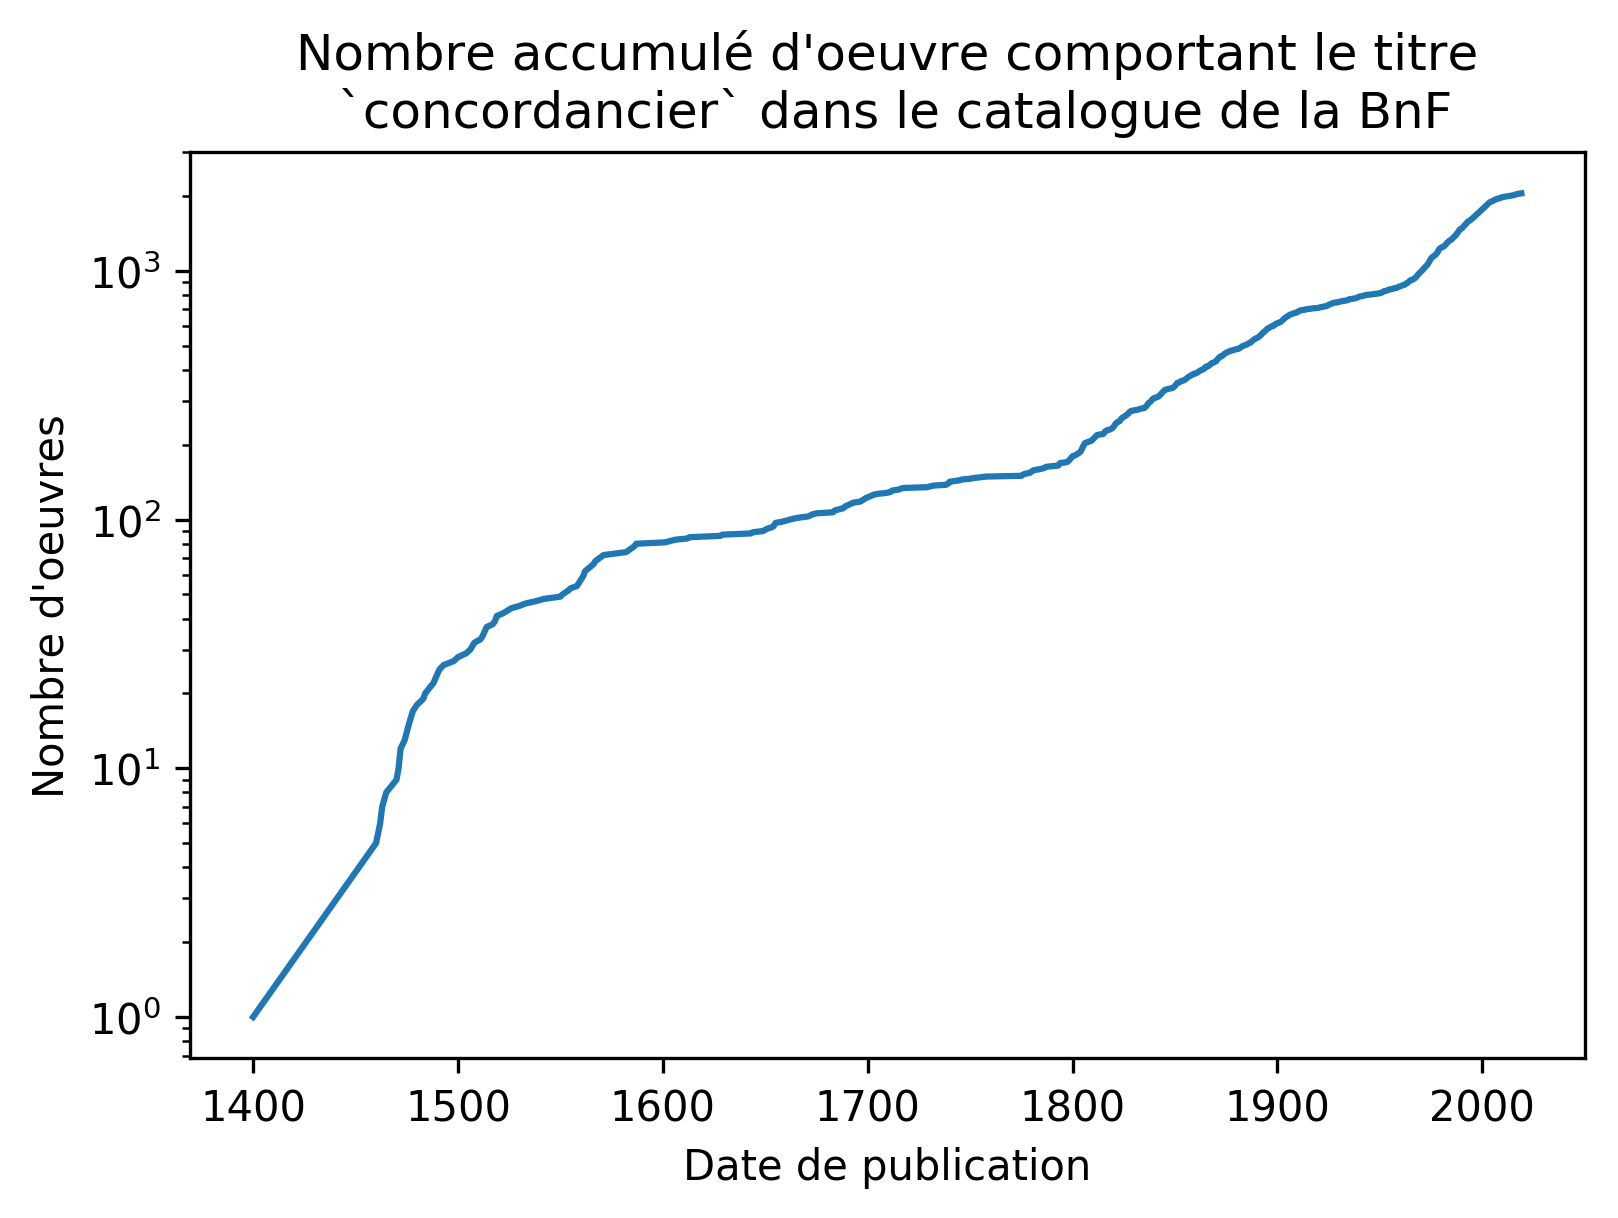
\includegraphics[width=10cm]{results/lemmatisation/histoire/concordanciers.png}
    \caption{Accumulation par dates de concordanciers conservés à la Bibliothèque Nationale de France}
    \label{lemmatisation:concordanciers}
\end{figure}

Et il ne s'agit pas que des concordances où le latin a été le premier à être lemmatisé de manière systématique pour une étude du langage. Dans le cadre du projet de Roberto Busa, à partir de 1949, on assiste à la première lemmatisation enregistrée numériquement (bien que sur des fiches perforées) via une collaboration avec IBM. Ce travail novateur aura pour but la constitution d'un corpus gigantesque de 11 millions de mots pour une publication vers 1980 de 56 volumes. Ce travail titanesque a une double particularité: il est vu comme l'un des projets fondateurs des humanités numériques; Roberto Busa est certainement aux humanités numériques ce que Thucydide et Hérodote sont à l'histoire, dans la méthode du premier comme dans le mythe personnel du second. Cette innovation est toute particulière mais ne connait pas d'impact direct: il faut attendre les années 60, attente que l'on peut - supposément - imputer à un besoin de croissance à la fois de l'accès à l'outil informatique (sans parler de démocratisation) et une croissance de la linguistique de corpus et la statistique textuelle (entre autres assistée par ordinateur). 

La première occurence universitaire d'un travail systématique de lemmatisation apparait avec le travail du LASLA, fondé le 13 septembre 1961\footcite{delatte_laboratoire_1961}. Dans leur article inaugural, les auteurs traitent de l'importance de la statistique en matière d'études stylistiques, et, partant d'un regret très simple, celui "d'*indices incomplets, inexacts ou même inexistants*", proposent un travail systématique d'annotation des textes latins. Cet article, bien qu'il porte de nombreuses critiques envers un possible manque de rigueur de certains philologues, montre surtout les opportunités, dans la continuité du travail des philologues, que porterait un tel outil, à savoir l'assurance de détecter des phénomènes non pas subjectivement ou intuitivement mais à partir de "comparaisons entre probabilités théoriques et fréquences réelles". Par ailleurs, l'article annonce la première étape du laboratoire, à savoir l'analyse des oeuvres de Sénèque. La perspective de Delatte et d'Évard est révolutionnaire, et la violence, à demi-voilée des propos \footnote{"Dans combien d'allitérations purement fortuites les commentateurs n'ont-ils pas voulu découvrir les intentions les plus subtiles", \cite[p.~442]{delatte_laboratoire_1961}}, rencontre très rapidement des phénomènes de résistance, ou, dans une perspective active, un système d'attaque pour faire changer une philologie percue comme figée dans un temps de l'avant-numérique. N. Perraux\footcite{perreaux_lemmatisation_2019}, dans une perspective d'histoire du domaine, a fait resurgir une polémique qui va en ce sens entre Pierre Grimal et Louis Delatte. Aux détours de quatres articles (\footcites{grimal_delatte_1964}{delatte_propos_1965}{grimal_index_1966}{delatte_index_1968}) dont deux sont des compte-rendus, les deux philologues engagent une "guerre franco-belge"\footcite{verdiere_pierre_1970}, initiée par P. Grimal, tournant autour de trois points principaux:
\begin{itemize}
    \item Sans aucun doute, une question de territoire intellectuel. P. Grimal tend à se positionner comme spécialiste français incontesté de Sénèque\footcite{verdiere_pierre_1970}, et, alors qu'il écrit une critique de l'index de L. Delatte publié en 1962, se prépare aussi à publier le sien. Dans le même contexte, quand L. Delatte fait une critique de la concordance de l'\textit{ad Marciam} de P. Grimal (publiée en 1965), il le fait aussi en défense de sa propre publication d'index de 1964.
    \item De manière sûre et certaine, il y a un débat sur la question de la concordance, conservant le contexte, contre l'index, répertoriant uniquement les passages de chaque lemme. Cette question de la forme, en dehors de toute méthode, est par ailleurs ravivée en 1979, quand L. Delatte et deux collègues\footcite{delatte_concordantiae_1979} viennent critiquer la concordance, générée automatiquement, de Roberto Busa de Sénèque.
    \item Enfin, et c'est un problème clair, une résistance complète et totale à la question du numérique de la part de P. Grimal. L. Delatte pose cependant un ensemble de jalons importants pendant les années soixante, non seulement en créant la \textit{Revue de l'Organisation Internationale pour l'Étude des Langues Anciennes par Ordinateur} \footnote{Aujourd'hui nommée Revue du LASLA. Autrefois abrégée RELO} mais en fondant sa pratique de la mécanographie sur un pilier simple: tout enregistrer pour pouvoir manipuler, statistiquement ou traditionnellement, des données en séries: "Le document de travail est, pour nous, le fichier de cartes perforées"\footcite[p~.202]{delatte_index_1968}. Au contraire, P. Grimal se réfugie tour à tour derrière des considérations très justes ("D’ailleurs, qui a son ordinateur personnel ?"\footcite[p.~111]{grimal_index_1966}) ou bien une incompréhension des possibilités de l'informatique:
    
    \blockquote{Renoncer à la machine, ce serait aussi se libérer d'un certain nombre de servitudes, comme l'adoption d'un code qui devient rapidement assez complexe lorsqu'on cherche à condenser un grand nombre de renseignements sur une fiche. La machine ne peut connaître que des catégories bien définies, chacune étant traduite par un symbole. Ces catégories constituent comme un quadrillage à l'intérieur duquel le réel doit entrer de gré ou de force, sans déborder d'une case dans l'autre\footcite[p.~131]{grimal_delatte_1964}}
\end{itemize}

Quoi qu'il en soit, si cette polémique, s'étirant sur une dizaine d'années, entre Liège et Paris, nous montre des formes de résistances et des questions quant aux nouvelles formes qui émergent, elle fait aussi resortir le travail titanesque qui se fait autour de L. Delatte et Étienne Évrard au LASLA. Il est y fait mention d'une "machine à lemmatiser" dès 1965\footcite{delatte_programme_1965} dont le fonctionnement sera la base pour tout ce qui se rapprocherait du lemmatiseur moderne, à savoir, pour une forme donnée, proposer l'ensemble des lemmes pouvant s'y rattacher, faisant tourner des rouages algorithmiques autour de quatres sets de données: les formes irrégulières, complètes, ne permettant aucune reconnexion; les radicaux; les terminaisons avec leurs codes morphologiques; les préfixes verbaux (ad-sum par exemple, afin de réduire la taille des calculs.). Cette base de lemmatiseur est la même que pour Words\footcite{whitaker_words_1993}, Morpheus\footcite{crane_generating_1991}, LEMLAT\footcite{bozzi_lemlat_1992} ou encore Analysis\footcite{ouvrard_analysis_1992} qui devient ensuite Collatinus\footcite{ouvrard_collatinus_1999}. Tous ces lemmatiseurs apparaissent au début des années 90, et deux sont issus du travail de passionnés, l'un professeur de latin (Yves Ouvrard) et l'autre colonel de l'armée étatsunienne \footnote{D'après sa nécrologie (\texttt{https://web.archive.org/web/20180705175913/https://www.findagrave.com/memorial/66889159}), il était en effet membre de la \textit{Defense Advanced Research Projects Agency} (DARPA) mais \textit{a priori} retraité au moment de la création de Words.}.

Cependant, si l'on retient pour lemmatiseur une définition stricte d'annotation par \textbf{un} lemme d'une forme, le premier lemmatiseur du latin vient bien plus tard. Et il ne s'agira pas d'un lemmatiseur du latin, mais bien de lemmatiseur en général: ce que Delatte estimait potentiellement impossible en 1968\footnote{"Un tel programme, supposant d'ailleurs une analyse conceptuelle, est très difficile sinon impossible à réaliser", \cite[p.~100]{delatte_index_1968}}), l'augmentation des puissances de calculs et de mémoire vive des ordinateurs a permis de le faire. À partir des années 1990, on voit apparaître des lemmatiseurs prenant en compte le contexte dans le choix des lemmes pour les formes ambivalentes. %(Insertion études par collatinus du nombre de lemme possible par forme ?). 
Dans ce contexte, les lemmatiseurs commencent à avoir besoin de données annotées (\textit{cf.} Chapitre Corpus [ToDO]). Parmi ceux-là, TreeTagger a, semble-t-il, reçu les faveurs de la communauté des lettres classiques et des latinistes médiévaux, bien qu'il ne soit \textit{a priori} pas le plus performant\footcite[Voir]{eger_lexicon-assisted_2015}. Plusieurs pistes sont à évoquer pour cette situation, sans qu'aucune preuve puisse être apportée. Il se pourrait que les phénomènes suivants aient fortement influencé sa place actuelle dans le domaine: son incorporation via TXM, sa prise en main relativement tôt dûe à son ainesse de presque 10 ans sur certains autres taggers, sa facilité d'installation, la constitution de modèles relativement tôt. 


\begin{figure}[h]
    \centering
    \resizebox{\textwidth}{!}{%
    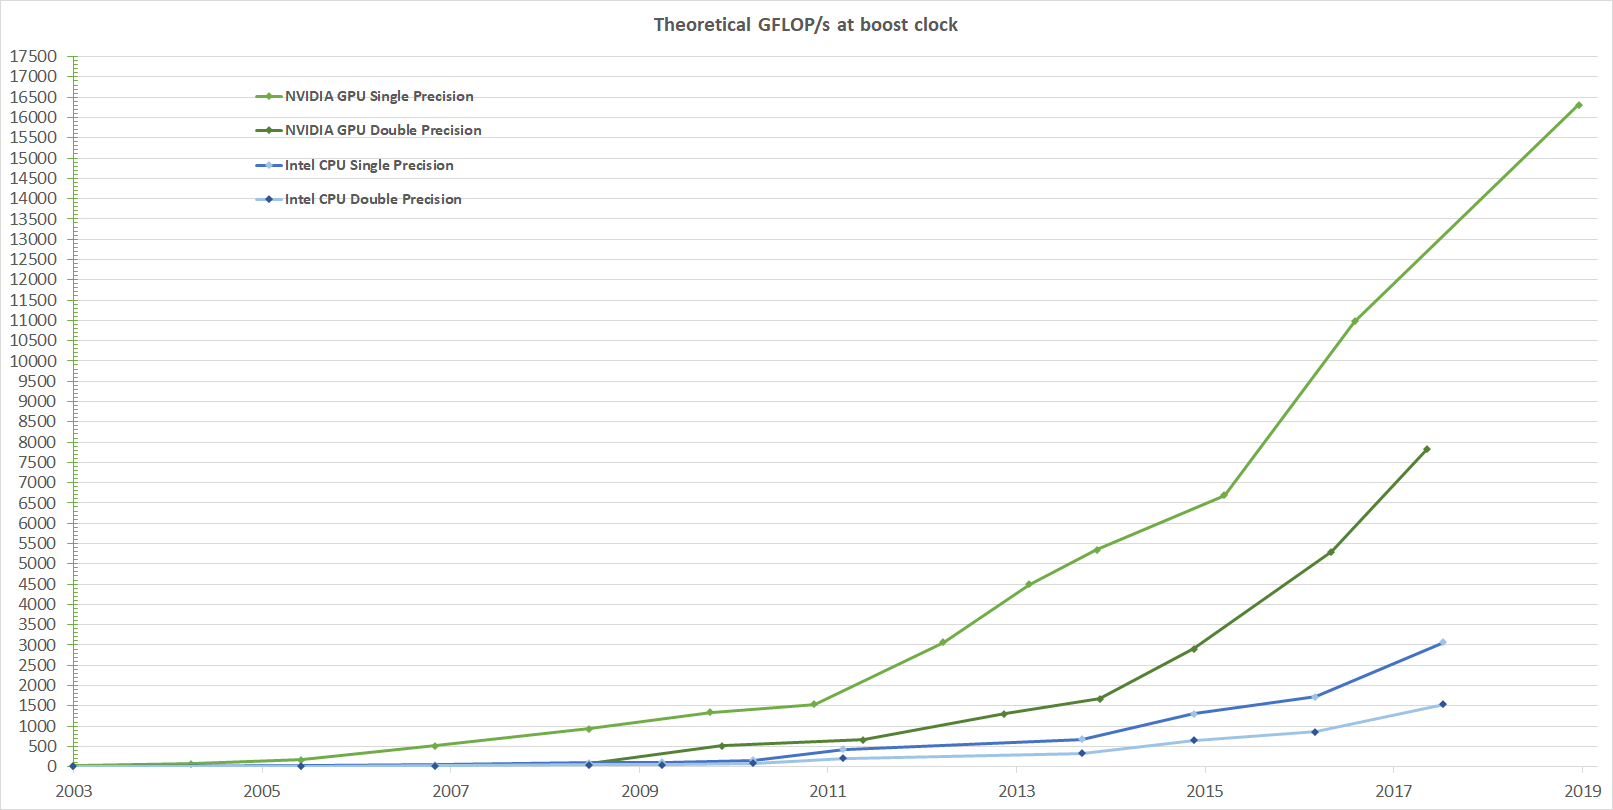
\includegraphics{results/lemmatisation/histoire/floating-point-operations-per-second.png}%
    }
    \caption{Opération à virgule flottante par seconde (FLOPS) entre processeur traditionnel (CPU) et de carte graphique (GPU). Source: \cite{noauthor_cuda_nodate}}
    \label{lemmatisation:histoire:puissance-gpu}
\end{figure}


Ces lemmatiseurs font face ensuite aux modèles complexes de \textit{deep learning} qui apparaissent au milieu et à la fin des années 2010, grâce à la montée en puissance encore des machines en calcul. En effet, dans un contexte de montée en puissance des cartes graphiques et de leurs GPUs (\textit{Graphical Processing Unit}, \textit{cf.} \ref{lemmatisation:histoire:puissance-gpu}), principalement poussée par une consommation du grand public de jeux vidéo\footcite{tanz_how_2017}, les chercheurs ont pu accéder à des machines beaucoup plus puissantes qu'auparavant pour des prix beaucoup plus faibles. En avril 2020, le prix d'une carte graphique professionnelle haut de gamme coûtait encore 7~602€ \footcite{noauthor_pny_2020} contre des prix variant de 1~149 à 1~899€ suivant les marques pour le haut de gamme particulier\footcite{noauthor_recherche_2020}\footnote{C'est sur ce modèle que l'ensemble des entraînements de cette thèse a été produit.}. Cette explosion de puissance, et sa démocratisation, permettent de prototyper ou d'assembler des machines de calcul à de plus nombreux laboratoires, permettant d'obtenir des différences en temps d'entraînement particulièrement importantes (la très grande majorité des calculs se faisant en opération à virgule flottante) permettant à la recherche d'essayer un plus grand nombre de combinaisons possibles de modèles (en 2017, d'après \ref{lemmatisation:histoire:puissance-gpu}, la différence de puissance est de x4). Cela permet à des projets comme Pandora \footcites{kestemont_lemmatization_2017}{de_gussem_integrated_2017}) puis Pie\footcite{manjavacas_improving_2019} de naître dans des laboratoires équipées de "petites" cartes graphiques. Enfin, parallèlement à cela, les géants du web investissent beaucoup dans des librairies de développement telles que PyTorch (Facebook) et Tensorflow (Google) qui permettent elles aussi de prototyper et de finaliser des modèles de prédiction, sans avoir à gérer la réimplémentation de modèles mathématiques complexes. 

\section{Les différents types d'outil}

\subsection{Les outils à base de règles (dès 1965)}

Dès 1965 et la création du LASLA donc, L. Delatte et É. Evrard cherchent à automatiser, en partie, la sélection des informations par lemmatisation automatique. Ce fonctionnement repose sur la constitution de plusieurs bases, qui correspondent majoritairement au fonctionnement des trois autres outils cités plus haut, à savoir Words de W. Whitaker, Morpheus de G. R. Crane, Collatinus de Y. Ouvrard (puis P. Verkerk à partir de 2015) ou encore, parmi les plus récents, LemLat: une base de lemmes, reliées à des bases de formes et de radicaux, permettent d'analyser des formes (\textit{cf.} \ref{lemmatisation:outils:collatinusAlgorythme} et \ref{lemmatisation:outils:collatinusAlgorythme} pour des exemples basés sur Collatinus). Chacun de ces lemmatiseurs est basé sur des dictionnaires différents, faisant état de traditions philologiques différentes en fonction des centres de recherche ou des nationalités. En effet, Word utilise l'Oxford Latin Dictionary, Morpheus utilise le Lewis \& Short, le LASLA utilise le Forcellini, Y. Ouvrard semble utiliser le Gaffiot, LemLat utilise principalement le Georges. Cette différence pose un problème de réconciliation de données que l'ERC LILA tente de régler en partie\footcite{mambrini_harmonizing_2019}. Dans cette catégorie de lemmatiseurs rentrent aussi les lemmatiseurs à dictionnaire de formes comme celui du CLTK\footcite{johnson2014cltk} qui enregistrent pour chaque forme connue les lemmes et les analyses possibles.

\begin{figure}[h]
    \centering
    \resizebox{\textwidth}{!}{%
    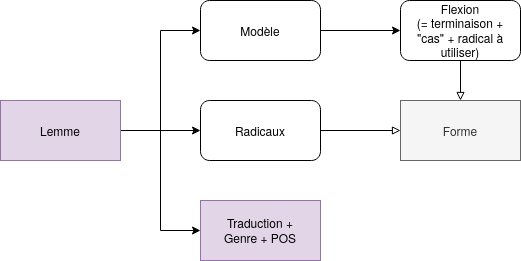
\includegraphics{results/lemmatisation/outils/CollatinusDB.png}%
    }
    \caption{Modèles de données dans Collatinus. Les formes sont générées et analysées à partir des flexions et radicaux, en fonction du modèle. }
    \label{lemmatisation:outils:collatinusDB}
\end{figure}


\begin{figure}[h]
    \centering
    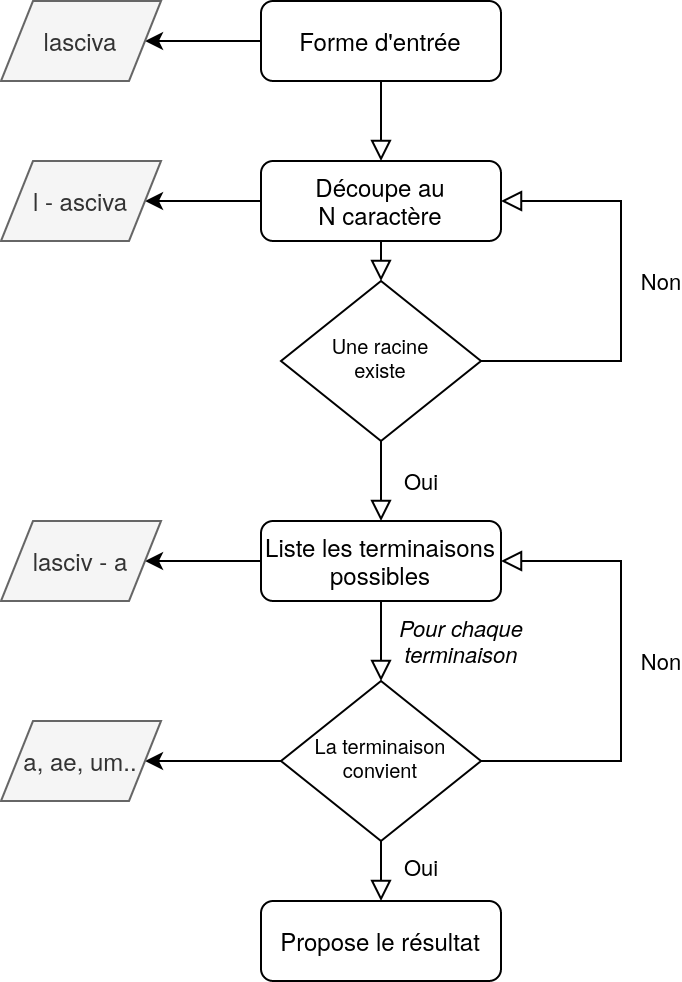
\includegraphics[width=6cm]{results/lemmatisation/outils/collatinus.png}
    \caption{Algorithme simplifié de Collatinus}
    \label{lemmatisation:outils:collatinusAlgorythme}
\end{figure}

L'avantage principal de ce genre de lemmatiseur consiste en sa capacité d'ingérer de nouveaux lemmes très facilement. Par exemple, dans Collatinus, \textit{lascivus} est donné par la ligne "lascīvus=lāscīvus|doctus|||a, um" où "a, um" est donné dans un but lexicographique mais n'a aucune utilité pour la génération des formes: seul "lascivus" et "doctus" (le modèle) suffisent pour cette partie de l'algorithme. Ainsi, pour ajouter un lemme "christianus", au cas où ce lemme tardif n'était pas inscrit dans le Gaffiot, il suffirait d'ajouter, scansion omise, "christianus|doctus|||a, um". À partir de ce simple ajout, la forme christiani sera nécessairement reconnue. Le désavantage de ces lemmatiseurs résident dans leur incapacité à faire le choix dans les analyses possibles, qu'il s'agisse des analyses morphologiques (lasciva est-il un nominatif singulier féminin ou un pluriel neutre ?) ou des choix de lemmes (ita est-il un adverbe ou la 2 éme personne du singulier présent impératif actif de ito, as, are ?).

\subsection{Les outils sur base statistique (1994 et après)}

Au milieu des années 90 mais surtout au début des années 2000 apparaissent les lemmatiseurs et analyseurs de POS tels que TreeTagger\footcite{schmid1994treetagger}, mais aussi TnT\footcite{brants_tnt_2000} et StanfordNLP\footcite{toutanova_feature-rich_2003}. Leurs modèles sont principalement basés sur des structures à base de probabilités d'occurrences de phénomènes en contexte, en intégrant la POS à l'analyse de lemme: on parle d'ailleurs principalement de POS-Tagger pour ces outils. Pour faire simple, ces taggers font usages de dictionnaires avec des fréquences possibles de POS affiliées, puis, en fonction en général de séquence de 3 à 4 mots, telle que "fortissimi sunt Belgae" pour "Horum omnium fortissimi sunt Belgae", ils cherchent à établir le tag le plus probable, avec des stratégies de décisions et d'éliminations diverses. TreeTagger change la donne en 1994 en apportant plusieurs modifications, qui probablement expliquent ses performances sur le latin. D'une part, TreeTagger constitue un dictionnaire de suffixes en plus du dictionnaire de forme, par ailleurs, pour faire face aux "\textit{ungrammaticalities}"\footcite[p.~2]{schmid1994treetagger} possibles de l'anglais, il attribue une probabilité minimale aux probabilités nulles. Dans le contexte d'une langue latine à l'ordre des mots non fixe et à la morphologie riche, ces deux facteurs pourraient expliquer une augmentation des scores importants comparés aux modèles précédents.

\begin{figure}[h]
    \centering
    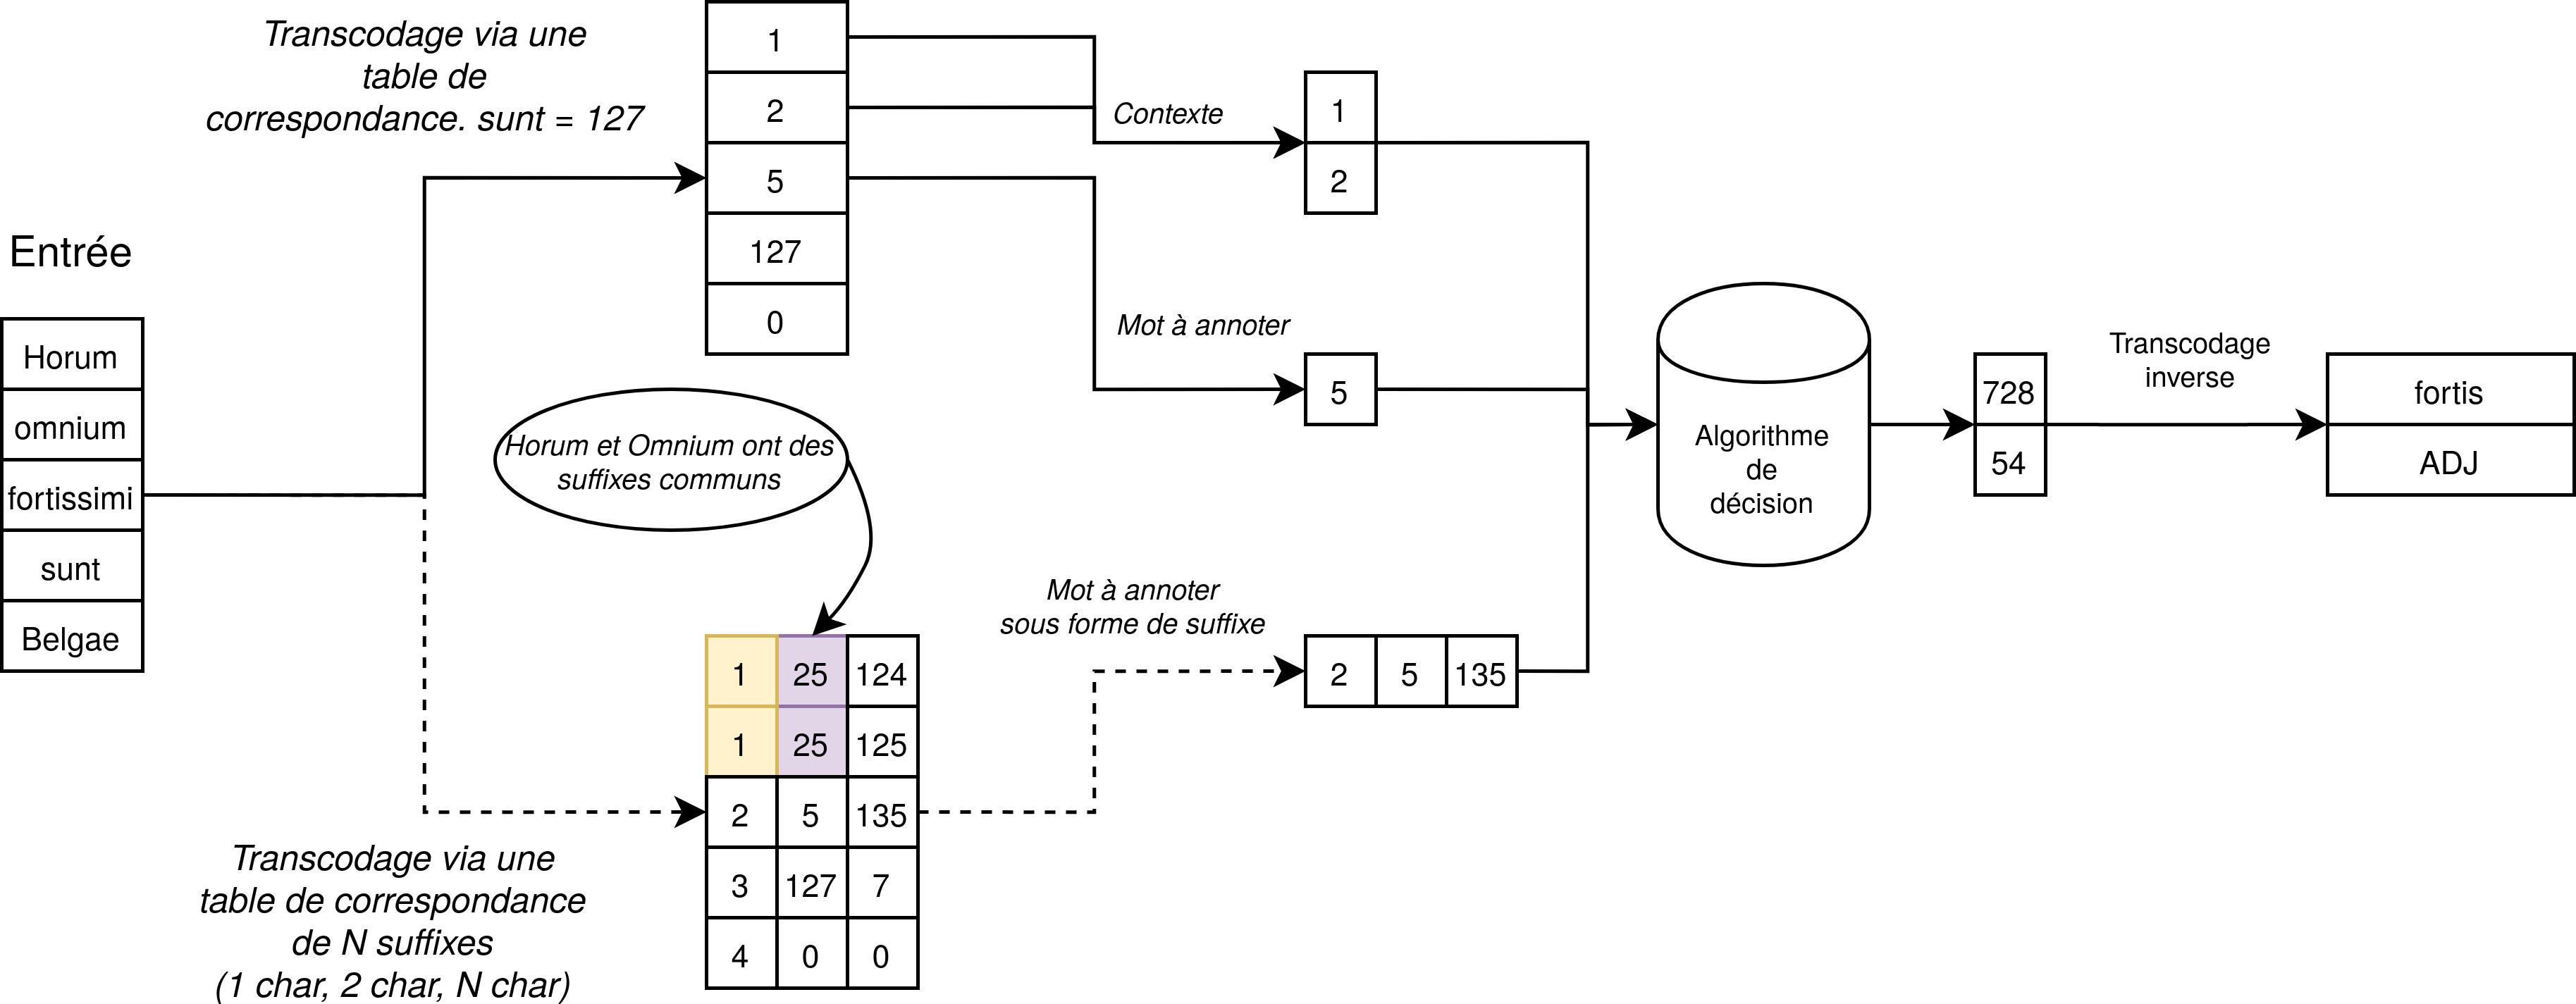
\includegraphics[width=\linewidth]{results/lemmatisation/outils/treetagger_type.png}
    \caption{Type de fonctionnement des outils de l'époque Treetagger. Une seule représentation des données est prise en compte au moment "d'un seul" calcul. Il s'agit principalement de modèles statistiques basés sur des probabilités d'apparition de phénomènes.}
    \label{lemmatisation:outils:type-treetagger}
\end{figure}

Le problème évident de ces lemmatiseurs reste aujourd'hui leur relation à un dictionnaire de forme et de lemmes qui ne leur permet pas (\textit{cf.} Figure \ref{lemmatisation:outils:type-treetagger}), en majorité, de prédire un lemme inconnu ou de gérer plus difficilement une forme inconnue en terme de lemmatisation. Les formes sont traitées telles quel, ce qui pose, même s'ils prennent en compte des suffixes, rapidement des problèmes pour la lemmatisation ou l'annotation POS dans le cadre du latin (avec des formes telles que -a communes à la fois aux noms, aux participes, aux adjectives, etc.).%exemple ? Vraiment difficile de savoir quoi dire ici...

\subsection{Les outils sur base de traduction (Milieu et fin des années 2010 et après)}

En 2016\footcite{kestemont_initial_2016}, Mike Kestemont propose une première version de Pandora\footcite{kestemont_lemmatization_2017}, un tagueur permettant à la fois la lemmatisation et l'annotation morpho-syntaxique. Sa particularité est de cibler le latin, à la fois médiéval et classique, en prenant en compte les difficultés inhérentes de la langue: d'une part, une morphologie très lourde, beaucoup plus lourde que celle de l'anglais par exemple; d'autre part, une syntaxe particulièrement libre. Ce travail est basé sur l'état de l'art en traitement automatique de la langue, à savoir des modèles d'apprentissage profond (\textit{deep learning}). Le modèle est constitué d'une couche d'embeddings, d'un encodeur LSTM et de plusieurs décodeurs fonctionnant soit sur une base LSTM (pour le lemme), soit sur une couche linéaire (pour les tâches morpho-syntaxique).


\begin{figure}[h]
    \centering
    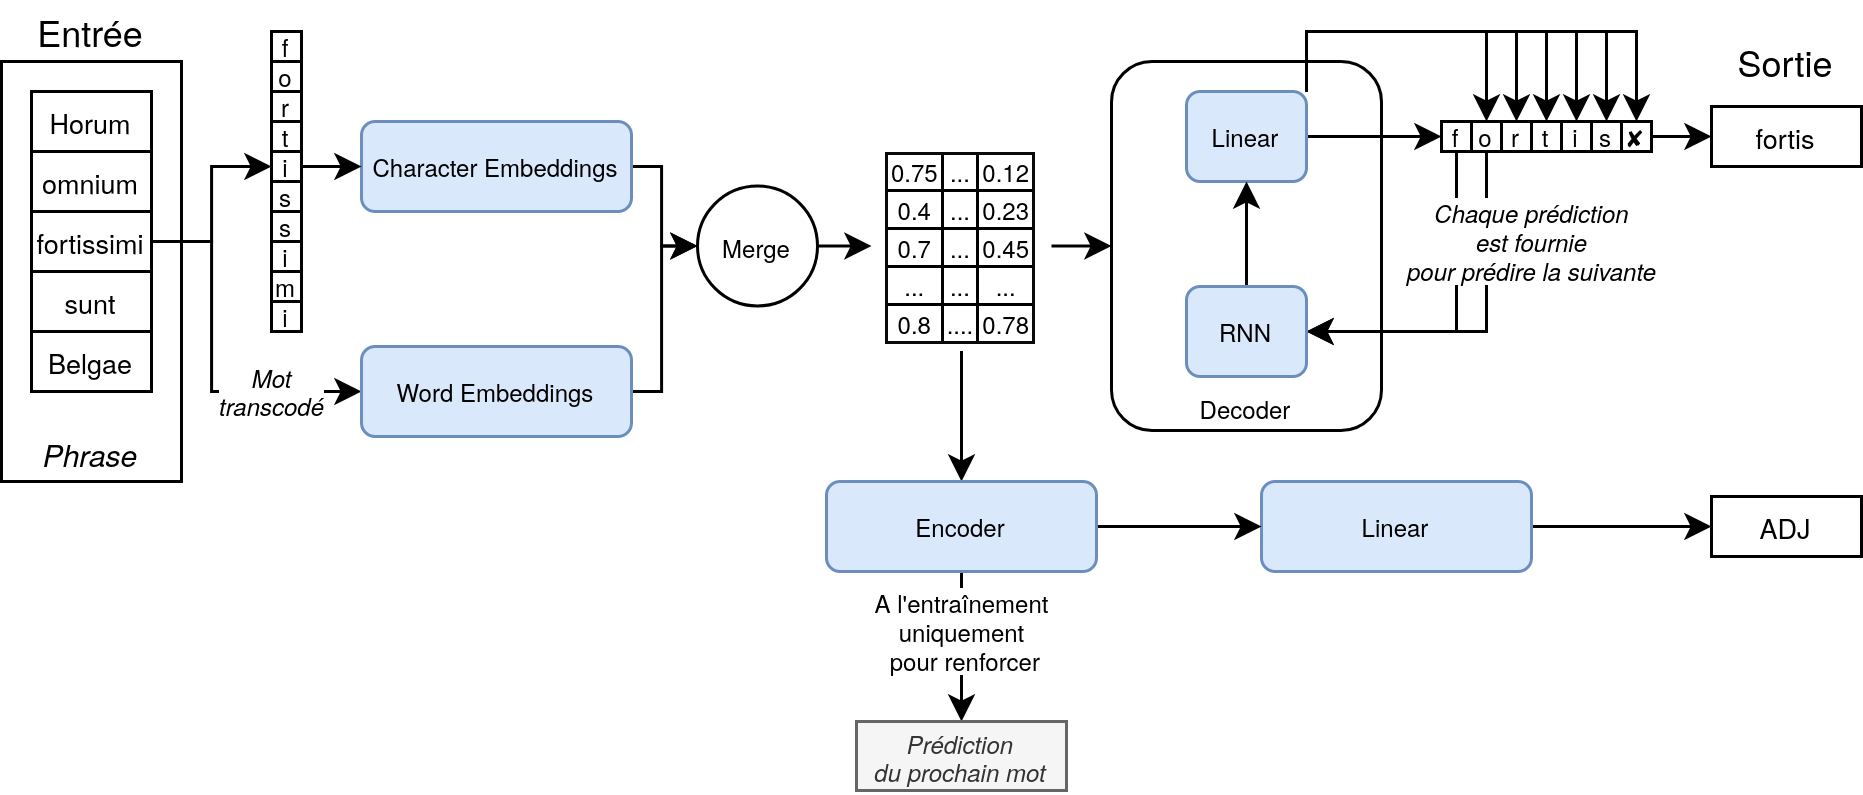
\includegraphics[width=\linewidth]{results/lemmatisation/outils/Pie.png}
    \caption{Représentation simplifiée de Pie. L'encodeur n'est utilisé que pour les classifications de mots et à l'entraînement comme support d'entraînement supplémentaire. Chaque lettre du lemme est prédite après l'autre vient un réseau acyclique. Bien que noté \textit{Embeddings}, le module de projection des caractères prend la forme au choix de CNN ou de RNN en plus d'une couche réelle d'Embeddings classiques}
    \label{lemmatisation:outils:pie}
\end{figure}

Ce lemmatiseur est perfectionné par E. Manjavacas\footcite{manjavacas_improving_2019} qui propose une architecture de code plus souple permettant entre autres de tester plusieurs configurations. Il apporte entre autre une meilleure gestion des caractères via des embeddings en CNN (plus rapide, aussi performant) et les modèles GRU pour les encodeurs et décodeurs. Le principe reste le même que pour la traduction automatique: au lieu de tenter de prédire des mots en anglais à partir des mots en français, \textit{pie} et les lemmatiseurs du même genre essaye de traduire chacune des lettres de la forme en lettres du lemme. De cette manière, il intègre des règles de lemmatisation telles que $\textrm{-ae} \rightarrow \textrm{-a}$. Cela signifie aussi que ce lemmatiseur peut avoir tendance à créer des lemmes inexistants, tout en respectant une certaine forme de logique interne: potentiellement, les lemmes ne sont pas les bons mais correspondent à ce que le lemmatiseur a estimé être une forme logique. % Faire une étude ici ?

\section{Corpus et méthodes d'évaluation}
\label{subsec:lemma_corpus}

\subsection{Les corpus disponibles}

Pour l'entraînement d'outils de lemmatisation, il existe très peu de corpus. On en compte quatre pour la période classique, utilisant deux dictionnaires de référence mais trois dictionnaire de POS. Ces trois corpus sont issus des projets Perseus, Proiel, Perseids et du LASLA. À l'exception de ce dernier, il sont tous primairement des corpus de treebank et non de lemmatisation: il semble qu'il n'y ait pas eu, historiquement, d'autres projets que ceux du LASLA pour la lemmatisation manuelle du latin classique.

Le corpus Perseus\footnote{Aussi connu sous le nom de \textit{Latin Dependency Treebank}} est un corpus dont l'article fondateur est publié en 2006\footcite{bamman_design_2006}. Au mois d'avril 2020, ce corpus contenait 76.670 tokens, ponctuations et enclitiques compris. L'objectif de ce projet d'annotation ne concerne en aucun cas la lemmatisation: d'ailleurs, le terme \textit{lemma} n'est présent qu'une seule fois pour près de 4000 mots et 10 pages de rédaction. Il est réalisé sous la direction de D. Bamman et G. Crane puis de G. Celano et de G. Crane. Sur les dernières années, la partie grecque du corpus a connu une croissance très importante, à l'opposé de la latine. Il ne comprend aucune oeuvre complète. Sa base de lemmes est dérivée du Lewis \& Short\footcite{shorts_latin_1958}.

Le corpus Harrington est un corpus issu d'une pratique pédagogique de l'annotation du latin\footcite{noauthor_harrington_nodate} via la plate-forme Perseids\footcite{almas_perseids_2016}. Il suit les mêmes recommandations en lemme et en morphologie que le corpus de Perseus, mais diffère sur la grammaire de dépendance utilisée. Certaines oeuvres de \textit{Perseus} sont réannotées avec cette grammaire, réduisant ainsi la taille du corpus utilisable de Perseus. Contrairement au corpus de Perseus, il est encore en cours de production par les étudiants de D. Harrington. Au mois d'avril 2020, il contenait 120~029 tokens, enclitiques et signes de ponctuation compris. Il ne comprend aucune oeuvre complète. 

Le corpus PROIEL est un corpus de projet plurilingue d'étude du \textit{Nouveau Testament} dans les langues indo-européennes anciennes\footcite{haug_creating_2008}. Il suit les mêmes recommandations en morphologie et en lemmatisation mais diffère sur ses annotations de POS et sur la grammaire de dépendance utilisée. Corpus toujours en actrivité, il ne comprend aucune oeuvre complète mais est assurément le corpus le plus important des trois issus du Lewis \& Short. Contrairement aux deux précédents, c'est un corpus qui, comme le LASLA, est d'abord un projet fondé par des linguistes et grammairiens avant d'être un produit de chercheurs en littératures ou d'enseignants comme G. Crane et D. Harrington\footnote{Nous parlons ici de fondation, G. Celano étant avant tout un linguiste.}.

\begin{table}[h]
\centering
\resizebox{\textwidth}{!}{%
\begin{tabular}{l|rrrrrr}
\toprule
        & Tokens             & Ponctuation & Nombre     & Nombre  & Lemmes & Dictionnaire \\ 
        &                    &   comprise  &  d'auteurs &  de textes & uniqes & \\   \midrule
PROIEL  & 225.064            & Non                  & 5                & 6  & 7246              & Lewis\\
Perseus & 79.670             & Oui                  & 12               & 12 & 6017              & Lewis \\
Harrington & 120.029             & Oui                  & 9               & 12 &  7675             & Lewis\\
LASLA   & \textbf{1.630.825} & Non                  & \textbf{18}                 &  \textbf{100+}     & 25135          & Forcellini \\ \bottomrule
\end{tabular}%
}
\caption{Résumé des informations sur les quatre corpus disponibles. Il existe 137 oeuvres au sens du LASLA, mais certaines sont des des découpes inhabituelles, nous préférons donc la notation 100+ ici.}
\label{tab:lemmatisation:corpus-entrainement}
\end{table}

Le corpus du LASLA, qui sera retenu de par sa taille et de par sa diversité, est un corpus dont nous avons précédemment parlé et dont la constitution a commencé dans les années 1960\footcites{delatte_laboratoire_1961}{BodsonCodification1966}. Contrairement aux autres corpus, il ne possède aucun texte à partir du 2e siècle de notre ère, ce qui en fait sa plus grande faiblesse. L'apprentissage machine reposant principalement sur le nombre de données et leur variété, il n'était pas envisageable de prendre un autre corpus. Par ailleurs, des essais en début de thèse nous avaient prouvé l'incapacité des modèles à prédire des résultats très fiables à partir des données de Perseus ou de Proiel.

\begin{figure}
    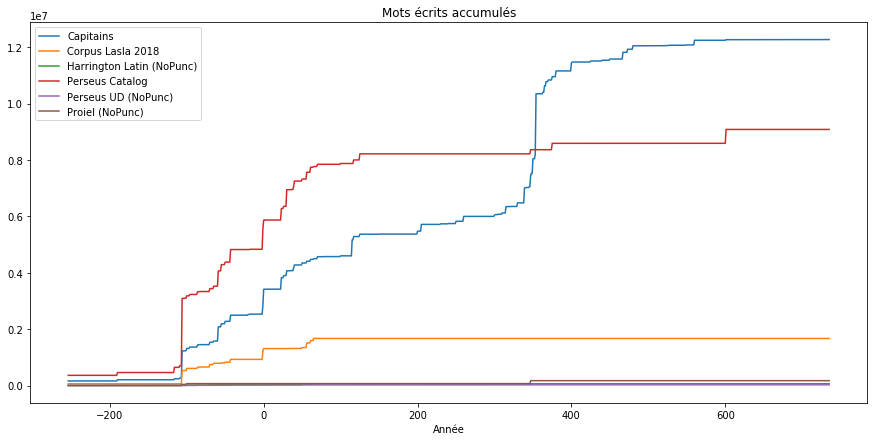
\includegraphics[width=\linewidth]{results/lemmatisation/corpus/tokens_per_year.png}
    \caption{Tokens accumulés, par année, en fonction des corpus latins bruts accessibles en open access (Capitains) ou du nombre estimés de par le Perseus Catalog.}
    \label{fig:lemmatisation:corpus-entrainement}
\end{figure}

\subsection{Le corpus du LASLA: choix d'étiquettage}

Le corpus du LASLA utilisé présente 1 630 825 mots dans la version à laquelle nous avons accès. Il est constitué de 25 135 lemmes, 1 008 types d'annotation morphologique (\textit{par exemple}  `Ablatif Pluriel` et `2eme personne Pluriel Indicatif Parfait Actif`) pour 28 grandes catégories syntaxiques (Nom, verbes, etc.) divisées là où il est possible de le faire en déclinaisons (nom1, nom2, etc.). On trouve dans le corpus de rares erreurs d'annotations, principalement des annotations incomplètes. Ces erreurs semblent marginales au regard du nombre de tokens. Le LASLA a fait le choix d'un étiquettage pour majeure partie morpho-syntaxique avec ici et là le choix de laisser des ambiguités. Nous revenons donc sur deux choix portant des conséquences sur les résultats de lemmatisation: d'une part, l'annotation du genre, d'autre part l'annotation des verbes à formes composées.

\newpara

Le LASLA a fait le choix de réserver \say{l'indication du genre pour les adjectifs, numéraux, les adjectifs-pronoms, les formes déclinées du verbe, hormis le gérondif}\footcite[p.~27]{BodsonCodification1966} dont la répartition est décrite en table \ref{table:lasla:genders-par-pos}. Ce choix a pour conséquence de laisser en partie le genre des noms inconnus: on ne pourra distinguer, dans le contexte de notre recherche, les noms par leur genre masculin ou féminin. On pourrait imaginer un travail de réannotation de tous les lemmes dont la POS est NOM avec leur genre quand il est fixe. Ce travail serait potentiellement riche d'influence sur les statistiques finales. Par ailleurs, le genre, à l'inverse du cas et du nombre, n'a pas été analysé en contexte (et donc syntaxiquement) mais en hors contexte (et donc morphologiquement), ce qui laisse des ambiguités comme \textit{bonum} qui est à la fois masculin et neutre à l'accusatif singulier. Dans ce contexte, le LASLA crée trois genres morphologiques supplémentaires des genres classiques: les genres Commun, Masculin-Féminin, Masculin-Neutre (dont la répartition dans le corpus d'entraînement est visible en \ref{table:lasla:genders-par-corpus}). L'explication derrière ce choix, disponible dans l'article de Bodson\footcite{BodsonCodification1966}, réside dans un problème technique de 1966, qui risquait de poser un problème d'export. Malheureusement, ce choix, aujourd'hui pourtant possible à résoudre, crée une forme de dette technique pour plus de 300 000 mots. On remarque cependant, à la marge, par alignement avec les formes possibles sur collatinus \footnote{\textit{Cf.} annexes numériques} qu'une analyse en contexte a été faite à la marge (\textit{cf.} table \ref{table:lasla:genders-alignement}).

\begin{table}[!htb]
    \begin{minipage}[t]{.4\linewidth}
        \centering
        \resizebox{\textwidth}{!}{%
            \begin{tabular}{l|rrr}
            \toprule
                     & PRO    & VER    & ADJ    \\ \midrule
            Com      & 30 004 & 14 841 & 26 384 \\
            Fem      & 37 177 & 16 393 & 34 292 \\
            Masc     & 42 598 & 18 785 & 24 331 \\
            MascFem  & 8 398  & 3 968  & 17 477 \\
            MascNeut & 25 459 & 12 170 & 30 815 \\
            Neut     & 46 479 & 11 151 & 25 381 \\ \bottomrule
            \end{tabular}
        }
        \caption{Répartition des genres par POS}
        \label{table:lasla:genders-par-pos}
    \end{minipage}% \quad
    \hspace{0.19\linewidth} 
    \begin{minipage}[t]{.4\linewidth}
        \centering
        \resizebox{\textwidth}{!}{%
            \begin{tabular}{l|rrr}
            \toprule
                       & Train   & Dev   & Test   \\ \midrule
            Fem        & 77 907   & 986   & 8 971   \\
            Masc       & 76 213   & 925   & 8 576   \\
            Neut       & 73 899   & 993   & 8 119   \\
            Com        & 63 304   & 789   & 7 136   \\
            MascFem    & 26 492   & 322   & 3 030   \\
            MascNeut   & 61 031   & 743   & 6 671   \\
            N/A        & 1 153 885 & 14 788 & 130 465 \\
            \textit{- Dont noms} & 433 117  & 5 634  & 48 840  \\ \bottomrule
            \end{tabular}
        }
        \caption{Répartition des genres par corpus}
        \label{table:lasla:genders-par-corpus}
    \end{minipage} 
\end{table}


\begin{table}[h]
\centering
\begin{tabular}{l|lll}
\toprule
         & MascNeut & MascFem & Com    \\ \midrule
0        & 783      & 653     & 1 478  \\
1        & 219      & 3 863   & 33     \\
2        & \textbf{65 852}   & \textbf{25 155}  & 2 512  \\
3        & 1 591    & 172     & \textbf{67 206} \\ \bottomrule
\end{tabular}
\caption{Nombre de genres possibles par alignement Forme+Cas+Nombre via PyCollatinus. Les informations qui ne sont pas en gras montrent une différence possible entre une annotation morphologique et morphosyntaxique. Il peut aussi s'agir d'erreurs de PyCollatinus.}
\label{table:lasla:genders-alignement}
\end{table}

\newpara

Un autre choix du LASLA a été d'annoter les participes avec le temps de la forme composée: pour amatus sum, amatus portera l'information du temps (parfait), du mode (indicatif), de la personne (1) et du genre (Masc) sans porter l'information du cas pourtant présent morphologiquement. Au contraire, \textit{sum} portera la simple annotation de verbe auxiliaire. Cela pose un problème de confusion pour une même forme amatus qui peut être annoté comme simple participe parfait passif avec une annotation Mode Voix Temps ajoutée à une annotation Genre Nombre Cas, et une forme amatus (elipse ou présence de) sum qui elle sera annotée aussi avec Mode Voix Temps mais le triplet Genre Nombre Personne. Dans cette optique, \textit{amatus} peut représenter 6 formes conjuguées hors participes, 7 pour le neutre \textit{amatum} (\textit{cf.} Table \ref{table:amatus_forms}). %
%
% Exemple pour le parfait passif
%
Ainsi, dans la phrase du \textit{De Amicitia} de Cicéron, \say{\textbf{uidetis} in tabella iam ante quanta \textbf{facta} labes primo Gabinia lege biennio post Cassia }, \textit{uidetis} est annoté à la 2ème personne du pluriel indicatif présent actif là où \textit{facta} est annoté à la 3ème du singulier subjonctif parfait passif. Si cette approche est particulièrement intéressante dans un contexte d'analyse morpho-syntaxique, elle est d'autant plus difficile à différencier d'un \textit{facta} nominatif pour un lemmatiseur automatique. Quelle différence en effet peut être faite dans la phrase \say{non oculi tacuere tui \textbf{conscriptaque} uino mensa nec in digitis littera nulla fuit} (Ovid. Her. 2.5.17 sqq.) avec le cas précédent ? % D'ailleurs, n'est-ce pas un raté ??

% Fin d'exemple

\newpara

\begin{table}[h]
\centering
\begin{tabular}{@{}lll@{}}
\toprule
Forme & Mode & Temps \\ \midrule
amatus (sum) & Indicatif & Parfait \\
amatus (eram) & Indicatif & Plus-que-parfait \\
amatus (ero) & Indicatif & Futur antérieur \\
amatus (sim) & Subjonctif & Parfait \\
amatus (essem) & Subjonctif & Plus-que-parfait \\
amatus (esse) & Infinitif & Parfait \\
amatum (iri) & Infinitif & Futur \\ \bottomrule
\end{tabular}
\caption{Annotations possible pour la forme \textit{amatus} dans le LASLA, hors participes}
\label{table:amatus_forms}
\end{table}

Cette multiplicité d'annotation peut rendre le travail de l'annotation automatique, car elle sous-entend une capacité pour le lemmatiseur de reconnaître les formes au nominatif utilisées de manière adjectivales des formes utilisées comme verbe principal ou verbe subordonné. Nous proposons en \ref{subsec:training:lasla-modification} une analyse de modifications pour une simplification du travail du modèle, en vue de la création d'un modèle morphologique et non morpho-syntaxique plus performant.

\newpara

Lemmes en diachronie, lemmes en synchronie: nocte, ablatif de nox ou adverbe ?

Majuscules uniquement aux noms propres et adjectifs "propres".

\section{Configurations évaluées et processus décisionnel}

\subsection{Arbre décisionnel d'entraînement.}




\subsection{Impact du choix d'étiquettage des formes passives ou déponentes composées}
\label{subsec:training:lasla-modification}

Le choix d'annoter des formes simples (les participes) par le temps de la forme composée provoque une difficulté d'apprentissage importante. En retirant du lot les formes adjectivales, le \gls{micro-average} des formes simples est de 0.9767 là où la même mesure pour les formes composées stagne à 0.7330. Par ailleurs, le \gls{macro-average} et l'\gls{ecart-type} montre ces disparités (\textit{cf.} Table \ref{table:lasla:formes-simples-formes-composees}). La déviation standard des temps simples peut-être majoritairement expliquée par des formes extrêmement rares comme l'impératif présent passif (1 occurence sur le corpus de test, 0 de précision) ce qui appuie l'importance des deux mesures de micro et de macro-average. Pour gérer ce problème, on propose de traduire les annotations automatiquement pour ces parfaits: les temps composés utilisant le parfait passif passent de \textsc{Mode-Temps-Voix} à \textsc{Par-Pft-Voix} (où voix correspondra donc à passif, déponent ou semi-déponent). Les modes composés de l'infinitif sont annotés avec le cas, il sera donc conservé. Les autres modes passent automatiquement au nominatif et perdent l'annotation de personne. Cette conversion double le nombre de participes futurs, augmente de moitié le nombre de participes parfaits passifs et n'a bien sûr aucune incidence sur les participes présents (\textit{cf.} Table \ref{table:lasla:correction-temps}.) Les résultats (Table \ref{table:lasla:formes-simples-formes-composees}) sont sans appel: l'intégralité des annotations de formes composées (qui correspondent désormais aux participes) connaissent un bond de 40 points en macro-average et 18 points en micro-average. L'écart-type reste fort dans la mesure où certaines classes sont trop rares ou fautives (par exemple, les éléments annotés syntaxiquement comme des participes futur passifs sont dans leur intégralité des participes parfaits passifs.). Les classes fautives restantes posent un problème mais leur poids dans l'entraînement est assez négligeable pour ne pas influer la reconnaissance des participes parfaits passifs, participes futurs actifs et participes présents actifs (Table \ref{table:lasla:main-particips}).

% ToDo: L'annotation de l'auxiliaire ?

\begin{table}[h]
\centering
\begin{tabular}{@{}l|r|lll|lll@{}}
\toprule
                                &         & \multicolumn{3}{l}{Pré-correction} & \multicolumn{3}{l}{Post-correction} \\ \midrule
Précision                       & Support & Macro    & Écart-Type   & Micro    & Macro     & Écart-Type   & Micro    \\ \midrule
Verbes (hors N/A)               & 39465   & 0.6524   & 0.3992       & 0.9336   & 0.9061    & 0.2233       & 0.9667   \\
Formes simples                  & 31254   & 0.9417   & 0.1679       & 0.9780   & 0.9417    & 0.1677       & 0.9786   \\
Formes Composées                & 7027    & 0.3570   & 0.3566       & 0.7378   & 0.7636    & 0.3810       & 0.9174   \\
- \textit{dont participe}       & 4946/7027    & 0.6430   & 0.3610       & 0.8087   & 0.7636    & 0.3810       & 0.9174   \\
Formes “adjectivales”           & 1173    & 0.9067   & 0.1539       & 0.9227   & 0.9378    & 0.0595       & 0.9433   \\ \bottomrule
\end{tabular}
\caption{\Gls{precision} en fonction des catégories de temps sur la base forme composée/simple et les scores de la table \ref{table:lasla:verb-scores}. Les formes autres correspondent au supin, au gérondif, et à l'adjectif verbal, les formes composées contiennent la catégorie participe.}
\label{table:lasla:formes-simples-formes-composees}
\end{table}

% Check participe futur passif ?

\begin{table}[h]
\centering
\begin{tabular}{l|rrr|rrr}
\toprule
 & \multicolumn{3}{c}{Pré-correction} & \multicolumn{3}{c}{Post-correction} \\ 
 & Test & Dev & Train & Test & Dev & Train \\ \midrule
Par-Fut-Act & 214 & 20 & 1726 & 445 & 46 & 3908 \\
Par-Fut-Dep & 14 & 1 & 121 & 30 & 2 & 209 \\
Par-Fut-Pass & 0 & 0 & 0 & 3 & 0 & 54 \\
Par-Fut-SemDep & 1 & 0 & 13 & 3 & 1 & 28 \\
Par-Perf-Act & 1 & 0 & 2 & 1 & 0 & 2 \\
Par-Perf-Dep & 363 & 32 & 3267 & 653 & 65 & 6203 \\
Par-Perf-Pass & 2927 & 309 & 25334 & 4391 & 526 & 38030 \\
Par-Perf-SemDep & 23 & 5 & 217 & 58 & 11 & 537 \\
Par-Pres-Act & 1210 & 137 & 10935 & 1210 & 137 & 10935 \\
Par-Pres-Dep & 188 & 20 & 1493 & 188 & 20 & 1493 \\
Par-Pres-Pass & 0 & 0 & 1 & 0 & 0 & 1 \\
Par-Pres-SemDep & 5 & 5 & 70 & 5 & 5 & 70 \\ \bottomrule
\end{tabular}
\caption{Résultats sur le décompte de participes des conversions automatiques temps composés vers participe. On remarque a posteriori au moins 2 lignes problématiques (Par-Perf-Act) et (Par-Pres-Pass). Le poids de cette erreur sur un macro-average sera important mais négligeable sur le micro-average}
\label{table:lasla:correction-temps}
\end{table}

\begin{table}[h]
\centering
\resizebox{\textwidth}{!}{%
\begin{tabular}{l|rrrr|rrrr}
\toprule
 & \multicolumn{4}{c}{Pré-correction}     & \multicolumn{4}{c}{Post-correction} \\ \midrule
              & Précision & Rappel        & F1-Score & Support & Précision     & Rappel        & F1-Score      & Support \\ \midrule
Par-Fut-Act   & 0.91      & 0.89          & 0.90     & 214     & \textbf{0.97} & \textbf{0.99} & \textbf{0.98} & 445     \\
Par-Perf-Pass & 0.76      & 0.83          & 0.79     & 2927    & \textbf{0.91} & \textbf{0.94} & \textbf{0.93} & 4391    \\
Par-Pres-Act  & 0.94      & \textbf{0.98} & 0.96     & 1210    & \textbf{0.95} & 0.96          & 0.96          & 1210    \\ \bottomrule
\end{tabular}{}%
}
\caption{Résultats sur les trois formes principales du participe. En dehors d'un avantage de 2 points sur le rappel des participes présents actifs, tous les autres scores connaissent une augmentation notable, malgré une augmentation nette du nombre de données à tester.}
\label{table:lasla:main-particips}
\end{table}

\section{Pie: extensibilité des résultats}

L'entraînement de Pie sur un corpus test donné nous informe de sa valeur sur le corpus en tant que tel. Se pose la question cependant de la capacité de nos modèles à s'appliquer à un corpus étranger, de quantifier l'impact d'une potentielle spécialisation. Pour étudier cet impact, nous proposons quatre expériences qui permettront d'évaluer l'impact de la taille du corpus d'entraînement, de sa variété en style et en genre, et enfin une étude hors-domaine s'appliquant d'abord à un texte important pour notre corpus, les Priapées, puis à des extraits de textes tardifs, le corpus du LASLA s'arrêtant avant la fin du premier siècle de notre ère..

\subsection{Évaluation sur des données hors-domaine}

Si les tests du modèles nous présentent un outil performant, au delà des 97\% de reconnaissance des lemmes, ils ne nous montrent qu'une face de son usage. En effet, la constitution du corpus de test est faites d'extraits non connus certes, mais d'extraits des même textes que les corpus d'entraînements. Ils ont donc une très forte probabilité de posséder les mêmes caractéristiques en terme de syntaxe, de vocabulaire, de coupes opérées par l'éditeur. Par ailleurs, ils posent un second problème qui est celui de la période couverte par le corpus d'origine, à savoir que l'auteur le plus tardif dans le corpus est Juvénal, puis Sénèque.

Dans ce contexte, on parle en apprentissage machine de données hors domaine, des données dont aucune partie ou trait de définition ne se trouvent dans le corpus d'entraînement. Pour cette étude, nous proposons deux corpus hors domaines, l'un constitué de l'ensemble des Priapées 1 à 78 d'après la numérotation de Baehrens, l'autre constitué de 10 textes d'auteurs tardifs, majoritairement chrétiens. Les \textit{Priapées} offrent un texte à l'extrême fin de notre corpus en terme de date\footcite{citroni_les_2008} et sont parmi les oeuvres non-étiquettées les plus portées sur le sexe. Par ailleurs, le style court tout particulier de cet ouvrage offrent aussi un grand nombre de sujets différents sur un corpus finalement assez réduit (environ 3~000 mots). Le second corpus\footcite{glaise_2020_corpus_tardif} est constitué de dix-neuf d'oeuvres de dix-sept auteurs, dont les passages (hors ponctuation) comptent \textit{a minima} 500 mots et dont les auteurs datent du deuxième siècle au neuvième de notre ère (Eginhard) avec une concentration plus forte autour du quatrième\footnote{Le corpus comprend précisément 1 auteur du 2e, 3 du 3e, 5 du 4e, 4 du 5e, 2 du 6e, 1 du 7e, 1 du 9e.}. Si la date de fin de ce corpus est plus tardive que les bornes que nous nous sommes posées, elles permettent d'évaluer tout de même la capacité du modèle à s'étendre dans le temps malgré un entraînement spécifique sur un corpus républicain et du haut empire, où les marques de la chrétienté sont de fait absentes.


\subsubsection{Résultats généraux}

Le modèle propose des résultats convaincants sur une très grande majorité des \textit{Priapées}. La particularité des Priapées tiennent, d'un point de vue statistiques, de leur très petite taille: une médiane à 30 mots sur les soixante-seize premiers poèmes et une moyenne à 40 à cause d'individu abérrants tels que le poème 51 (150 mots) et 68 (237)\footnote{Au niveau des quartiles, 25\% des \textit{priapées} font moins de 24 mots, 75\% en font moins de 68. Toutes les tailles ne concernent que les mots, hors ponctuation donc mais incluant les clitiques.}. L'\textit{accuracy} peut donc grandement varier d'un texte à l'autre, une erreur pouvant représenter au pire une chute de 9\% d'un score\footnote{C'est le cas potentiellement des \textit{priapées} 13, 59 et 62 dans notre édition.} ou au mieux 0.4\% pour la plus grande priapée. Les résultats restent plus qu'honorable, avec une chute d'uniquement trois points par rapport au corpus de test principal et une accuracy globale de 94.2\% sur la tâche de lemmatisation (\textit{cf.} table \ref{tab:out_of_domain_global_accuracy} et figure \ref{fig:priapea_varations_boxplot}). Certaines priapées ont des scores particulièrement bas qui ne semblent pas avoir de lien avec leur taille: on notera ainsi les priapées 75 (82 mots, 84\%) et 46 (45 mots, 84\%) qui se trouvent dans la moyenne haute des tailles de poème.

Comme le corpus des \textit{Priapées}, le corpus de latin tardif propose des résultats avec une faible perte, de l'ordre de trois points aussi. L'ensemble des autres annotations performent globalement mieux que sur les \textit{Priapées} (annotation `cas` à 92.9\% contre 89.4\%) ce qui peut potentiellement s'expliquer par la forme poétique et courte des épigrammes qui ne laisse pas une grande place à l'erreur. Dans ce corpus, deux textes font office de résultats aberrants, à savoir Jérôme, \textit{Commentaire sur Jérémie} et Grégroire de Tours, \textit{Historia Francum} qui chutent respectivement à 87 et 88\%. Les textes ont majoritairement la même taille, aux alentours de 500 à 600 mots, avec Commodien, \textit{Instructiones} comme texte le plus court (412 mots) et Augustin, \textit{De Civitate Dei} ainsi que Hilaire de Poitiers, \textit{Tractatus super psalmos} comme texte extrêmement longs\footnote{L'export des textes à corriger ayant allongé les textes involontairement, et l'annotation ayant été corrigée, l'ensemble de ces textes a tout de même été conservé, produisant de fait un écart avec la moyenne de 500 mots.}.

\begin{table}[h]
    \centering
    \begin{tabular}{l|rr|rr}
    \toprule
         Catégorie &  \multicolumn{2}{c}{\textit{Accuracy}} & \multicolumn{2}{c}{\textit{Accuracy quand applicable}} \\
    \midrule    
                {} &  Priapées &    Tardif                  & Priapées &    Tardif                                   \\
    \midrule
             lemma &     0.942 &    0.945                   &   N/A    &    N/A                                      \\
               Deg &     0.968 &    0.975                   &   0.903  &    0.915                                    \\
              Numb &     0.947 &    0.965                   &   0.941  &    0.964                                    \\
            Person &     0.990 &    0.997                   &   0.960  &    0.991                                    \\
Mood\_Tense\_Voice &     0.961 &    0.977                   &   0.870  &    0.923                                    \\
              Case &     0.894 &    0.929                   &   0.841  &    0.880                                    \\
              Gend &     0.917 &    0.928                   &   0.778  &    0.792                                    \\
               pos &     0.950 &    0.676                   &   N/A    &    N/A                                      \\
    \bottomrule
    \end{tabular}
    \caption{Résultat du modèle sélectionné sur le corpus des priapées et de latin tardif. L'accuracy quand applicable désigne la précision de l'algorithme sur les termes qui nécessitent une annotation, en d'autres termes, pour la personne par exemple, seuls les annotations sur les verbes sont concernées.}
    \label{tab:out_of_domain_global_accuracy}
\end{table}


\begin{figure}[ht]
    \centering
    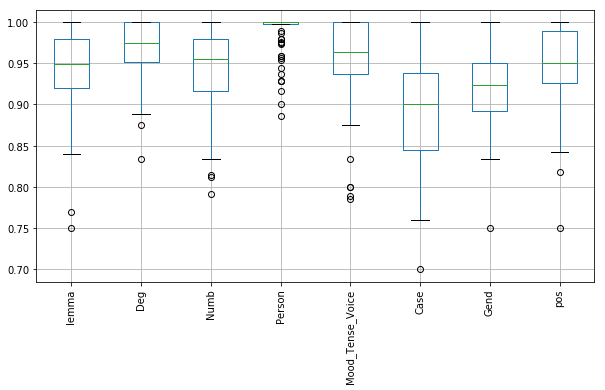
\includegraphics[width=0.7\linewidth]{results/lemmatisation/extensibilite/PriapeaBoxPlot.png}
    \caption{Variation des taux d'erreurs sur l'ensemble du corpus des \textit{Priapées}}
    \label{fig:priapea_varations_boxplot}
\end{figure}

\subsubsection{Étude des erreurs}

Si ces chiffres annoncent potentiellement une très bonne nouvelle pour la période tardive et les sujets qui nous intéressent, ne s'attarder que sur une échelle quantitative macro serait une erreur de taille. Si la loi de Zipf s'applique logiquement, on sait que les termes les plus fréquents représentent une très grosse partie du corpus final: sur le corpus latin tardif, sur 15~188 formes, 4~908 formes dépendent de 34 lemmes qui apparaissent au minimum plus de 100 fois\footnote{Il s'agit du quantile 0.99 du corpus.}. Parmi ces lemmes, seuls 3 sont des verbes (\textit{sum}, \textit{dico}, \textit{facio}) et 3 des noms communs (\textit{deus}, \textit{dominus}, \textit{filius}); seuls les noms présentent une particularité thématique, les trois verbes étant particulièrement important dans la langue latine en général.

\begin{figure}
    \centering
    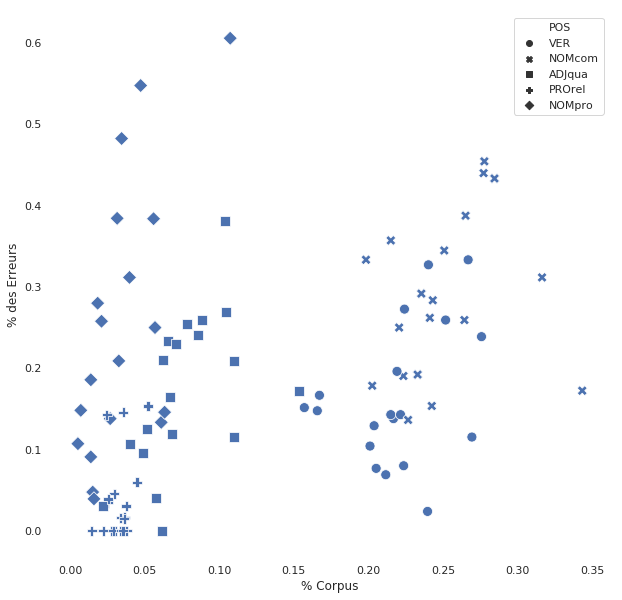
\includegraphics[width=0.5\linewidth]{results/lemmatisation/extensibilite/LatinTardifPosError.png}
    \caption{Responsabilité des POS dans les erreurs du lemmatiseur. Chaque point représente un texte.}
    \label{fig:latin_tardif_error_pos}
\end{figure}

On trouve bien des erreurs typiques du lemmatiseur, en regardant celles-ci de plus près: erreur du type lemme \textit{debeo} à la place du nom \textit{debitum}, erreur de déclinaison et de formation de la racine telle que \textit{terrenus} à la place de \textit{terrena}, majuscule oubliée dans les noms propres avec \textit{uenus}/\textit{Uenus}, orthographe du lemme réactionnaire (\textit{Aggaeus} pour \textit{Aggeus}). À la lecture des erreurs, on se rend compte d'une potentielle surreprésentation des noms propres dans les lemmes mal annotés et dont la racine supposée est fausse, capitalisation comprise: on notera par exemple \textit{Ierusalem/Hierusalis}, \textit{Hieremias/Hieremia}, \textit{Babylonius/Babylonii} chez Jérôme. La grande majorité des mots alors mal annotés partagent les traits suivant:

\begin{itemize}
    \item le lemme est issu de la langue grecque ou hébreuse: \textit{Christus}, \textit{Israel}, \textit{Pascha}, \textit{Dauid}.
    \item le lemme possède une variation graphique latine forte, chose inconnue dans le corpus classique, telles que \textit{Bethleem}/\textit{Bethlehem}, \textit{Hierusalem}/\textit{Ierusalem}
\end{itemize}

\subsection{Étude de l'impact de la taille du corpus sur l'efficacité du modèle}
\label{lemmatisation:extensibilite:tailles}

Pour la première expérience, nous voulons évaluer l'impact de la taille d'un corpus sur les différents éléments de mesure à notre disposition. Nous proposons donc des coupes de corpus du corpus LASLA à 1\%, 5\%, 7.5\%, 10\%, 20\%, 40\%, et enfin 80\% du corpus. Dans chacun des corpus d'entraînement, le corpus de développement représentera lui aussi, 10\% de la portion de corpus utilisée pour l'entraînement. La découpe se fait au niveau de chacun des fichiers d'entraînement du LASLA, à savoir un découpage au niveau de l'oeuvre (\textit{Poésie} de Catulle) ou à un sous-niveau de l'oeuvre (César, \textit{Guerre des Gaules}, 1). Chaque découpe du corpus connait alors la même variété d'auteur, la même variété de genre et de thème. Les découpes sont prises aléatoirement dans les séquences constituées par le LASLA. Nous mesurons trois tâches, à savoir:

\begin{itemize}
    \item la tâche lemma, qui indique une compréhension du vocabulaire, de la syntaxe et de la morphologie,
    \item la tâche POS, qui indique une compréhension morpho-syntaxique
    \item la tâche Gend, qui indique une compréhension de la morphologie.
\end{itemize}

Durant l'entraînement, le modèle principal ayant obtenu les meilleurs résultats sur le corpus global a montré des faiblesses sur les corpus de petites tailles. Pour chaque corpus, deux configurations ont donc été testées, une avec un module GRU simple couche (RNN=1) et un module GRU double couche (RNN=2) pour la partie de caractère embeddings. Les résultats (\textit{cf.} Table \ref{tab:percent_corpus_comparaison}) montrent que l'augmentation de la taille du corpus avec une même variété de genres et d'auteurs a un impact fort (plus de 1 point de gagné) jusqu'à l'utilisation de 40 \% du corpus, quelque soit, ou presque\footnote{Il existe en effet un valeurs aberrantes pour le genre et la POS pour le passage de 7.5\% du corpus à 10\% du corpus.}. Au contraire, les passage de 40\% à 60\% du corpus et de 60\% à 80\% ne représentent des gains que de 0.23 et 0.46 points respectivement, et donc, un passage de 96.79\% d'accuracy pour le corpus à 40\% à seulement 97.48\% pour le corpus à 80\%, pour un doublement du nombre de tokens annotés utilisés pour l'entraînement, soit une augmentation d'environ 600~000 tokens (passage de 622~238 tokens d'entraînement à 1~226~227).


\begin{table}[]
    \centering
    \begin{tabular}{lrrrrrrrr}
    \toprule
RNN &  \% Corpus &   Lemme &  Gain Lemme &     POS &  Gain POS &    Genre &  Gain Genre \\
\midrule
1 &     0.010 &  0.7408 &      0.0000 &  0.7907 &    0.0000 &  0.8508 &     0.0000 \\
1 &     0.050 &  0.8895 &      0.1487 &  0.8868 &    0.0961 &  0.9025 &     0.0517 \\
2 &     0.075 &  0.9209 &      0.0314 &  0.9206 &    0.0338 &  0.9302 &     0.0277 \\
2 &     0.100 &  0.9363 &      0.0154 &  0.9288 &    0.0082 &  0.9332 &     0.0030 \\
2 &     0.200 &  0.9492 &      0.0129 &  0.9474 &    0.0186 &  0.9484 &     0.0152 \\
2 &     0.400 &  0.9679 &      0.0187 &  0.9609 &    0.0135 &  0.9609 &     0.0125 \\
2 &     0.600 &  0.9702 &      0.0023 &  0.9637 &    0.0028 &  0.9645 &     0.0036 \\
2 &     0.800 &  0.9748 &      0.0046 &  0.9660 &    0.0023 &  0.9697 &     0.0052 \\
    \bottomrule
    \end{tabular}
    \caption{Résultat des tests sur un corpus de test de 140~000 mots représentant 80\% du corpus de test original. RNN correspond au nombre de couches du module d'encodage des caractères. Les mesures de gain correspondent à la différence avec le modèle précédent, il faut donc lire "Le modèle à 80\% du corpus performe 0.46 points de plus que le modèle à 60\% du corpus."}
    \label{tab:percent_corpus_comparaison}
\end{table}

D'après ces résultats, on peut penser que le lemmatiseur apprend "assez" de la richesse de vocabulaire et de la syntaxe d'un auteur pour s'enrichir jusqu'à environ 40\% de ses textes. Une stratégie de création de corpus pourrait donc se focaliser sur l'annotation d'extraits d'auteurs, plutôt qu'une approche d'annotation complète. Cependant, on peut aussi voir les gains minimes comme de véritables bonds en valeur absolue: si, pour un corpus de 10 millions de tokens, les résultats passent de 96.09\% d'accuracy à 96.97\%, et que ces résultats se retransmettent de manière régulière, le nombre d'erreurs passe de 391~000 à 303~000, soit une chute de 88~000 erreurs.



\begin{comment}
\subsection{Taille et diversité: corpus Perseus}
\label{lemmatisation:extensibilite:perseus}

Nous avons vu en \ref{subsec:treebank_corpora} que le corpus de Perseus pour le treebank, mis en forme pour le projet Universal Dependencies (\Gls{UD}), présente un corpus comprenant peu de textes et peu de mots comparé au corpus du LASLA (26 000 mots contre 1.7 millions) mais cependant une variété de style et d'époque assez forte parmi les corpus de ce genre.

\newpara

Pour compléter l'analyse précédente \ref{lemmatisation:extensibilite:tailles}, on reproduit un corpus similaire à celui de Perseus, dans la limite où 4 oeuvres présentes dans ce dernier ne le sont pas dans le corpus LASLA, à savoir les \textit{Fables} de Phèdres, les \textit{Res Gestae} d'Auguste, la \textit{Vie d'Auguste} de Suétone, la \textit{Vulgate} de Jérôme. On propose de remplacer pour le même nombre de phrases par deux autres oeuvres \footnote{Ces oeuvres sont mentionnées dans le corpus de Perseus original mais n'ont pas été nettoyées pour le projet \Glspl{UD})} à savoir les \textit{Fastes} d'Ovides et le \textit{Satyricon} de Pétrone. Le corpus d'entraînement, de développement et de test sont constitués à partir du seul corpus d'entraînement en \ref{lemmatisation:extensibilite:tailles}: les séquences sont prises aléatoirement, sans prendre en compte la position de la séquence dans l'oeuvre originale de Perseus, l'équivalent de 10\% et 20\% du nombres de phrases en entraînement sont utilisées pour le corpus spécifique de développement et de test (ci-après \texttt{perseus-test}). Le résultat de cette génération de corpus donne 1361 séquences contre 1334 originellement, mais surtout une forte augmentation du nombre de mots 26 081 contre 18 184 démontrant des tailles de séquences plus grandes dans le corpus LASLA (\textit{cf.} tables \ref{table:perseus-ud:chunks-and-tokens}, \ref{table:lasla:perseus-ud}).  Pour l'évaluation, nous proposons à la fois le résultat sur un corpus \texttt{perseus-test} qui représente la même diversité d'oeuvres, mais aussi le corpus test utilisés pour nos mesures. Nous n'évaluons que les tâches \texttt{lemma}, \texttt{pos} et \texttt{Gend} pour les raisons mentionnées plus haut. 

\newpara

% Analyse des résultats

\begin{table}[h]
\centering
\begin{tabular}{lll}
\toprule
 Title                  & Chunks & Tokens \\ \midrule
 Auguste, Res Gestae    & 38     & 708    \\
 Caesar                 & 24     & 352    \\
 Cicero, In Catilinam   & 137    & 1897   \\
 Phèdre, Fables         & 233    & 2397   \\
 Properce               & 224    & 2776   \\
 Salluste, Catilina     & 336    & 4999   \\
 Suétone, Vie d'Auguste & 109    & 2046   \\
 Tacite, Histoires      & 64     & 866    \\
 Virgile, Énéide        & 15     & 142    \\
 Vulgate                & 154    & 2001   \\ \midrule
 Total                  & 1334   & 18184  \\ \bottomrule
\hline
\end{tabular}
\caption{Répartition par oeuvres du nombres de séquences et de tokens dans le corpus Perseus UD 2.1}
\label{table:perseus-ud:chunks-and-tokens}
\end{table}

\begin{table}[h]
\centering
\resizebox{\textwidth}{!}{%
\begin{tabular}{l|llll|llll}
\toprule
                  & \multicolumn{4}{l}{Test Perseus}        & \multicolumn{4}{l}{Test LASLA}          \\ 
                  & Accuracy & Précision & Recall & Support & Accuracy & Précision & Recall & Support \\ \midrule
\textbf{Lemma}    &          &           &        &         &          &           &        &         \\
\textit{Tous}     & 0.6550   & 0.2864    & 0.2919 & 5754    & 0.6132   & 0.0990    & 0.0858 & 172968  \\
\textit{Inconnus} & 0.0306   & 0.0094    & 0.0155 & 1534    & 0.7480   & 0.2760    & 0.2438 & 12790   \\
\textit{Ambigus}  & 0.7558   & 0.4873    & 0.5027 & 434     & 0.019    & 0.0035    & 0.0061 & 53069   \\ \midrule
\textbf{POS}      &          &           &        &         &          &           &        &         \\
\textit{Tous}     & 0.8427   & 0.7991    & 0.7482 & 5754    & 0.8183   & 0.6831    & 0.6062 & 172968  \\
\textit{Inconnus} & 0.5913   & 0.0947    & 0.0790 & 1534    & 0.7835   & 0.5866    & 0.5358 & 12790   \\
\textit{Ambigus}  & 0.7672   & 0.5453    & 0.5678 & 799     & 0.5671   & 0.0755    & 0.0691 & 53069   \\ \midrule
\textbf{Gender}   &          &           &        &         &          &           &        &         \\ 
\textit{Tous}     & 0.8637   & 0.8448    & 0.6139 & 5754    & 0.8646   & 0.6315    & 0.4288 & 172968  \\
\textit{Inconnus} & 0.6780   & 0.2043    & 0.1463 & 1534    & 0.6604   & 0.6981    & 0.6698 & 12790   \\
\textit{Ambigus}  & 0.6506   & 0.7027    & 0.6620 & 538     & 0.7067   & 0.1615    & 0.1274 & 53069   \\ \bottomrule
\end{tabular}%
}
\caption{Évaluation d'un modèle linéaire entraîné sur le corpus \texttt{perseus-train} (26 081 tokens, 9 textes) dans Pie contre un corpus test de Perseus et un corpus LASLA plus générique (les modèles avec decodeur plafonnant à 0 pour la tâche \texttt{lemma})}
\label{table:lemmatisation:perseus-scores}
\end{table}

\end{comment}

\subsection{Variation de genre, variation de style}
\label{lemmatisation:extensibilite:prose-vers}

Afin d'aller encore plus loin dans l'analyse de l'effet du corpus, nous proposons de reproduire les principes de l'étude de C. Poudat et D. Longrée\footcite{poudat2009variations}. Dans cette étude, les auteurs analysent l'impact de l'unicité de genre, de style, chronologique sur l'entrainement de tagger automatiques, en particulier TreeTagger cité plus haut. L'expérience repose sur les comparaisons suivantes:
\begin{itemize}
    \item Style d'ouvrage contre style d'auteur (César, Guerre des Gaules; César, Guerre Civile)
    \item Style d'auteur contre style de genre (César; Pseudo-César et Salluste)
    \item Style du genre à travers le temps (César, Pseudo-César et Salluste; Quinte-Curce et Tacite)
    \item Style de la prose à l'épreuve des variations génériques (histoire; traités, dialogues)
    \item Style de la prose contre le vers
\end{itemize}{}

Cependant, il nous semble important de dévier sur les corpus utilisés et constitués: les corpus constitués dans le cadre de cette évaluation présentent une très grande variation de taille. Or, dans le contexte d'une modélisation, et de l'impact de ces traits (à savoir genre, style, période), il ne semble pas souhaitable de comparer des entraînements effectués sur 52~000 tokens contre des modèles entraînés sur près de 400~000 tokens\footcite[par exemple, p.~135, 2.~2.~4]{poudat2009variations}. Nous reprenons donc les grandes lignes et constituons 4 sous-expériences.

\begin{itemize}
    \item Une première expérience, sur de petits corpus en vers (environ 90~000 tokens), permettra d'identifier l'impact d'un auteur dans un modèle, ou d'une époque: un corpus double Horace \& Lucrèce (91~555 tokens, 6 oeuvres différentes), un Virgile (87488 tokens), un Ovide (95~409 tokens).
    \item Une seconde expérience, sur des corpus plus larges (environ 117~000 tokens), permettra d'étudier l'impact du genre avec deux corpus Sénèque (\textit{Ad Lucilium}, 118~801 tokens; Autres oeuvres philosophies, 117~550 tokens), un corpus mixte théâtre Sénèque et Plaute (115~571 tokens, 16 oeuvres), un corpus Cicéron court (116~367 tokens, 2 oeuvres), un corpus Tacite (117~552 tokens, 4 oeuvres).
    \item Une troisième exprérience cherchera à analyser l'impact du mode de rédaction (vers contre prose) sur l'extensibilité des résultats avec un corpus Prose (257 034 tokens, 7 auteurs, 9 oeuvres) et un corpus Vers (259 717 tokens, 7 auteurs, 17 oeuvres).
    \item Une quatrième expérience portant sur des corpus de 390~000 tokens profitera de la richesse du corpus de Cicéron, en évaluant l'impact de la diversité d'auteurs (corpus divers, 392~402 tokens, 13 auteurs, 24 textes) contre celle de la diversité d'oeuvres d'un même auteur (corpus Cicéron Discours, 391~390 tokens, 1 auteur, 44 oeuvres)\footnote{On peut retrouver le découpage dans la table en annexe \textbf{A FAIRE}}.
\end{itemize}{}

Les oeuvres de test sont toujours prises en hors domaine, à savoir qu'elles ne peuvent pas faire partie des mêmes oeuvres que les oeuvres d'entraînement. Dans la mesure du possible, elles sont aussi issues de corpus d'auteurs différents (\textit{cf.} Table \ref{table:lemmatisation:extensibilite:test-corpus}).

\begin{table}
\resizebox{\textwidth}{!}{%
\begin{tabular}{lll|ll|r|l}
    \toprule
     Auteur & Oeuvre & Passage & Genre & Tokens & Auteur présent dans corpus \\ \midrule
     César & Guerre des Gaules & 3 & Histoire & 3 637 & Prose \\
     Catulle & Poésie & Complet & Poésie & 13 020 & \\
     Cicéron & De l'Amitié & Complet & Traité & 9 272 & Cicéron Petit \\
     &&&&& Cicéron Discours \\
     &&&&& Prose \\
     Cicéron & Catilinaires & 1 & Traité & 9 272 & \textit{idem} \\
     Quinte Curce & Histoires & 3 & Histoire & 7 175 & Prose \\
     &&&&& Divers \\
     Horace & Épodes & Complet & Poésie & 3 071 & Vers \\
     &&&&& Horace+Lucrèce \\
     &&&&& Corpus Divers \\
     Ovide & Ibis & Complet & Poésie &  4 196 & Vers \\
     &&&&& Ovide \\
     &&&&& Corpus Divers \\
     Salluste & Catilina & Complet & Histoire & 10 598 & \\
     Sénèque & De la brièveté de la vie & Complet & Dialogues & 6113 & Sénèque (Les 3) \\
     &&&&& Prose \\
     &&&&& Divers \\
     Sénèque & Médée & Complet & Tragédie & 5 685 & \textit{idem} \\
     Tacite & Germanie & Complet & Histoire & 5 648 & Prose \\
     &&&&& Tacite \\
     &&&&& Divers \\ \bottomrule
\end{tabular}%
}%
     \caption{Oeuvres et nombre de tokens pour le test }
     \label{table:lemmatisation:extensibilite:test-corpus}
\end{table}

\section{Alignement Vulgate}

Problème des hapaxes ET des noms hébreux et grecs.

\quote{Et ipse Jesus erat incipiens quasi annorum triginta, ut putabatur, filius Joseph, qui  \\fuit Heli, qui fuit Mathat, \\
qui fuit Levi, qui fuit Melchi, qui fuit Janne, qui fuit Joseph, \\
qui fuit Mathathiæ, qui fuit Amos, qui fuit Nahum, qui fuit Hesli, qui fuit Nagge, \\
qui fuit Mahath, qui fuit Mathathiæ, qui fuit Semei, qui fuit Joseph, qui fuit Juda, \\
qui fuit Joanna, qui fuit Resa, qui fuit Zorobabel, qui fuit Salatheil, qui fuit Neri, \\
qui fuit Melchi, qui fuit Addi, qui fuit Cosan, qui fuit Elmadan, qui fuit Her, \\
qui fuit Jesu, qui fuit Eliezer, qui fuit Jorim, qui fuit Mathat, qui fuit Levi, \\
qui fuit Simeon, qui fuit Juda, qui fuit Joseph, qui fuit Jona, qui fuit Eliakim, \\
qui fuit Melea, qui fuit Menna, qui fuit Mathatha, qui fuit Natham, qui fuit David, \\
qui fuit Jesse, qui fuit Obed, qui fuit Booz, qui fuit Salmon, qui fuit Naasson, \\
qui fuit Aminadab, qui fuit Aram, qui fuit Esron, qui fuit Phares, qui fuit Judæ, \\
qui fuit Jacob, qui fuit Isaac, qui fuit Abrahæ, qui fuit Thare, qui fuit Nachor, \\
qui fuit Sarug, qui fuit Ragau, qui fuit Phaleg, qui fuit Heber, qui fuit Sale, \\
qui fuit Cainan, qui fuit Arphaxad, qui fuit Sem, qui fuit Noë, qui fuit Lamech, \\
qui fuit Methusale, qui fuit Henoch, qui fuit Jared, qui fuit Malaleel, qui fuit Cainan, \\
qui fuit Henos, qui fuit Seth, qui fuit Adam, qui fuit Dei.}

\subsection{Analyse exploratoire et tentative d'interprétation}

Projection 2D des embeddings ?


\section{Analyse des résultats}
\label{subsec:lemma_resultats}

\begin{table}[]
\begin{tabular}{@{}llll@{}}
\toprule
lemma     & prediction & token      & number \\ \midrule
Christus  & Christi    & Christi    & 10     \\
unum      & unus       & unum       & 10     \\
qui       & quod       & quod       & 9      \\
Ierusalem & Hierusalis & Hierusalem & 8      \\
quod      & qui        & quod       & 7      \\
Dauid     & Dauidis    & Dauid      & 6      \\
Christus  & Christis   & Christi    & 5      \\
caelus    & caelum     & caelos     & 4      \\
Christus  & Christius  & Christi    & 4      \\
christus  & Christus   & Christum   & 4      \\
debitum   & debeo      & debitum    & 4      \\
Iesus     & iesum      & Iesum      & 4      \\
is        & eo         & eo         & 4      \\
Israel    & Israceles  & Israhel    & 4      \\
minoro    & minor      & minorati   & 4      \\
Abram     & aber       & Abram      & 3      \\ \bottomrule
\end{tabular}
\end{table}

\section{Étiquetage automatique du corpus}


Chaque lemmatiseur ont quoiqu'il arrive une idée de la langue. Dans le cadre de l'annotation du latin, cela se trouve par exemple dans la différenciation ou non des lettres u/v et i/j dans les formes d'entrées. Dans ce cadre, il faut alors adapter la forme d'entrée au lemmatiseur afin d'éviter à tout prix une incapacité à traiter les données, tout simplement parce qu'elles n'ont pas été prévues. % A lire


\begin{table}[]
\begin{tabular}{l|rrrr}
\hline
                                          & A                 & B                 & C              & D              \\ \hline
Normalisation des lettres                 & Non               & Oui               & Non            & Oui            \\
Suppression des formes inconnues (points) & Non               & Non               & Non            & Oui            \\
Tokenization Phrase                       & Ponctuation Forte & Ponctuation Forte & 35 Mots        & 35 Mots        \\ \hline
lemma              & \textbf{-1.51} & -0.22          & \textbf{-1.62} & -0.23 \\
Deg                & -0.30          & -0.16          & -0.26          & -0.06 \\
Numb               & -0.41          & -0.31          & -0.56          & -0.12 \\
Person             & -0.05          & 0.00           & -0.06          & -0.03 \\
Mood\_Tense\_Voice & -0.11          & -0.02          & -0.12          & -0.04 \\
Case               & \textbf{-0.76} & \textbf{-0.66} & \textbf{-1.41} & -0.32 \\
Gend               & -0.28          & -0.13          & -0.23          & -0.11 \\
pos                & \textbf{-0.57} & -0.33          & \textbf{-0.66} & -0.18 \\ \hline
\end{tabular}
\end{table}